%% abtex2-modelo-trabalho-academico.tex, v-1.9.7 laurocesar
%% Copyright 2012-2018 by abnTeX2 group at http://www.abntex.net.br/ 
%%
%% This work may be distributed and/or modified under the
%% conditions of the LaTeX Project Public License, either version 1.3
%% of this license or (at your option) any later version.
%% The latest version of this license is in
%%   http://www.latex-project.org/lppl.txt
%% and version 1.3 or later is part of all distributions of LaTeX
%% version 2005/12/01 or later.
%%
%% This work has the LPPL maintenance status `maintained'.
%% 
%% The Current Maintainer of this work is the abnTeX2 team, led
%% by Lauro César Araujo. Further information are available on 
%% http://www.abntex.net.br/
%%
%% This work consists of the files abntex2-modelo-trabalho-academico.tex,
%% abntex2-modelo-include-comandos and abntex2-modelo-references.bib
%%

% ------------------------------------------------------------------------
% ------------------------------------------------------------------------
% abnTeX2: Modelo de Trabalho Academico (tese de doutorado, dissertacao de
% mestrado e trabalhos monograficos em geral) em conformidade com 
% ABNT NBR 14724:2011: Informacao e documentacao - Trabalhos academicos -
% Apresentacao
% ------------------------------------------------------------------------
% ------------------------------------------------------------------------

\documentclass[
% -- opções da classe memoir --
12pt,				% tamanho da fonte
openright,			% capítulos começam em pág ímpar (insere página vazia caso preciso)
twoside,			% para impressão em recto e verso. Oposto a oneside
a4paper,			% tamanho do papel. 
% -- opções da classe abntex2 --
%chapter=TITLE,		% títulos de capítulos convertidos em letras maiúsculas
%section=TITLE,		% títulos de seções convertidos em letras maiúsculas
%subsection=TITLE,	% títulos de subseções convertidos em letras maiúsculas
%subsubsection=TITLE,% títulos de subsubseções convertidos em letras maiúsculas
% -- opções do pacote babel --
english,			% idioma adicional para hifenização
french,				% idioma adicional para hifenização
spanish,			% idioma adicional para hifenização
brazil				% o último idioma é o principal do documento
]{abntex2}

% ---
% Pacotes básicos 
% ---
\usepackage{lmodern}			% Usa a fonte Latin Modern			
\usepackage[T1]{fontenc}		% Selecao de codigos de fonte.
\usepackage[utf8]{inputenc}		% Codificacao do documento (conversão automática dos acentos)
\usepackage{indentfirst}		% Indenta o primeiro parágrafo de cada seção.
\usepackage{color}				% Controle das cores
\usepackage{graphicx}			% Inclusão de gráficos
\usepackage{microtype} 			% para melhorias de justificação
% ---

% ---
% Pacotes adicionais, usados apenas no âmbito do Modelo Canônico do abnteX2
% ---
\usepackage{lipsum}				% para geração de dummy text
% ---

% ---
% Meu pacotes individuais
% ---
\usepackage{amsmath}
\usepackage{amsfonts}
\usepackage{booktabs}
\usepackage{siunitx}
\usepackage{multirow}
\usepackage{color,soul}
 
% ---
% Pacotes de citações
% ---
\usepackage[brazilian,hyperpageref]{backref}	 % Paginas com as citações na bibl
\usepackage[alf]{abntex2cite}	% Citações padrão ABNT

% --- 
% CONFIGURAÇÕES DE PACOTES
% --- 

% ---
% Configurações do pacote backref
% Usado sem a opção hyperpageref de backref
\renewcommand{\backrefpagesname}{Citado na(s) página(s):~}
% Texto padrão antes do número das páginas
\renewcommand{\backref}{}
% Define os textos da citação
\renewcommand*{\backrefalt}[4]{
	\ifcase #1 %
	Nenhuma citação no texto.%
	\or
	Citado na página #2.%
	\else
	Citado #1 vezes nas páginas #2.%
	\fi}%
% ---

% ---
% Informações de dados para CAPA e FOLHA DE ROSTO
% ---
\titulo{Mensurando Autoritarismo nas Palavras: o caso da Câmara dos Deputados no Brasil}
\autor{Marcio de Lucas Cunha Gomes}
\local{Brasil}
\data{2020}
\orientador{Nara Pavão}
\coorientador{}
\instituicao{%
	Universidade Federal de Pernambuco -- UFPE
	\par
	Departamento de Ciência Política
	\par
	Programa de Pós-Graduação}
\tipotrabalho{Dissertação (Mestrado)}
% O preambulo deve conter o tipo do trabalho, o objetivo, 
% o nome da instituição e a área de concentração 
\preambulo{Dissertação apresentada ao Departamento de Ciência Política da Universidade  Federal de Pernambuco para obtenção  do  título  de  Mestre em Ciência Política. Orientadora: Prof. Dra. Nara Pavão}
% ---


% ---
% Configurações de aparência do PDF final

% alterando o aspecto da cor azul
\definecolor{blue}{RGB}{41,5,195}

% informações do PDF
\makeatletter
\hypersetup{
	%pagebackref=true,
	pdftitle={\@title}, 
	pdfauthor={\@author},
	pdfsubject={\imprimirpreambulo},
	pdfcreator={LaTeX with abnTeX2},
	pdfkeywords={abnt}{latex}{abntex}{abntex2}{trabalho acadêmico}, 
	colorlinks=true,       		% false: boxed links; true: colored links
	linkcolor=blue,          	% color of internal links
	citecolor=blue,        		% color of links to bibliography
	filecolor=magenta,      		% color of file links
	urlcolor=blue,
	bookmarksdepth=4
}
\makeatother
% --- 

% ---
% Posiciona figuras e tabelas no topo da página quando adicionadas sozinhas
% em um página em branco. Ver https://github.com/abntex/abntex2/issues/170
\makeatletter
\setlength{\@fptop}{5pt} % Set distance from top of page to first float
\makeatother
% ---

% ---
% Possibilita criação de Quadros e Lista de quadros.
% Ver https://github.com/abntex/abntex2/issues/176
%
\newcommand{\quadroname}{Quadro}
\newcommand{\listofquadrosname}{Lista de quadros}

\newfloat[chapter]{quadro}{loq}{\quadroname}
\newlistof{listofquadros}{loq}{\listofquadrosname}
\newlistentry{quadro}{loq}{0}

% configurações para atender às regras da ABNT
\setfloatadjustment{quadro}{\centering}
\counterwithout{quadro}{chapter}
\renewcommand{\cftquadroname}{\quadroname\space} 
\renewcommand*{\cftquadroaftersnum}{\hfill--\hfill}

\setfloatlocations{quadro}{hbtp} % Ver https://github.com/abntex/abntex2/issues/176
% ---

% --- 
% Espaçamentos entre linhas e parágrafos 
% --- 

% O tamanho do parágrafo é dado por:
\setlength{\parindent}{1.3cm}

% Controle do espaçamento entre um parágrafo e outro:
\setlength{\parskip}{0.2cm}  % tente também \onelineskip

% ---
% compila o indice
% ---
\makeindex
% ---

% ----
% Início do documento
% ----
\begin{document}
	
	% Seleciona o idioma do documento (conforme pacotes do babel)
	%\selectlanguage{english}
	\selectlanguage{brazil}
	
	% Retira espaço extra obsoleto entre as frases.
	\frenchspacing 
	
	% ----------------------------------------------------------
	% ELEMENTOS PRÉ-TEXTUAIS
	% ----------------------------------------------------------
	% \pretextual
	
	% ---
	% Capa
	% ---
	\imprimircapa
	% ---
	
	% ---
	% Folha de rosto
	% (o * indica que haverá a ficha bibliográfica)
	% ---
	\imprimirfolhaderosto*
	% ---
	
	% ---
	% Inserir a ficha bibliografica
	% ---
	
	% Isto é um exemplo de Ficha Catalográfica, ou ``Dados internacionais de
	% catalogação-na-publicação''. Você pode utilizar este modelo como referência. 
	% Porém, provavelmente a biblioteca da sua universidade lhe fornecerá um PDF
	% com a ficha catalográfica definitiva após a defesa do trabalho. Quando estiver
	% com o documento, salve-o como PDF no diretório do seu projeto e substitua todo
	% o conteúdo de implementação deste arquivo pelo comando abaixo:
	%
	% \begin{fichacatalografica}
	%     \includepdf{fig_ficha_catalografica.pdf}
	% \end{fichacatalografica}

\begin{fichacatalografica}
\sffamily
\vspace*{\fill}					% Posição vertical
\begin{center}					% Minipage Centralizado
	\fbox{\begin{minipage}[c][8cm]{13.5cm}		% Largura
			\small
			\imprimirautor
			%Sobrenome, Nome do autor
			
			\hspace{0.5cm} \imprimirtitulo  / \imprimirautor. --
			\imprimirlocal, \imprimirdata-
			
			\hspace{0.5cm} \thelastpage p. : il. (algumas color.) ; 30 cm.\\
			
			\hspace{0.5cm} \imprimirorientadorRotulo~\imprimirorientador\\
			
			\hspace{0.5cm}
			\parbox[t]{\textwidth}{\imprimirtipotrabalho~--~\imprimirinstituicao,
				\imprimirdata.}\\
			
			\hspace{0.5cm}
			1. Palavra-chave1.
			2. Palavra-chave2.
			2. Palavra-chave3.
			I. Orientador.
			II. Universidade xxx.
			III. Faculdade de xxx.
			IV. Título 			
		\end{minipage}}
	\end{center}
\end{fichacatalografica}
% ---


% ---
% Inserir folha de aprovação
% ---

% Isto é um exemplo de Folha de aprovação, elemento obrigatório da NBR
% 14724/2011 (seção 4.2.1.3). Você pode utilizar este modelo até a aprovação
% do trabalho. Após isso, substitua todo o conteúdo deste arquivo por uma
% imagem da página assinada pela banca com o comando abaixo:
%
% \begin{folhadeaprovacao}
% \includepdf{folhadeaprovacao_final.pdf}
% \end{folhadeaprovacao}
%
\begin{folhadeaprovacao}
	
	\begin{center}
		{\ABNTEXchapterfont\large\imprimirautor}
		
		\vspace*{\fill}\vspace*{\fill}
		\begin{center}
			\ABNTEXchapterfont\bfseries\Large\imprimirtitulo
		\end{center}
		\vspace*{\fill}
		
		\hspace{.45\textwidth}
		\begin{minipage}{.5\textwidth}
			\imprimirpreambulo
		\end{minipage}%
		\vspace*{\fill}
	\end{center}
	
	Trabalho aprovado. \imprimirlocal, 01 de março de 2020:
	
	\assinatura{\textbf{\imprimirorientador} \\ Orientador} 
	\assinatura{\textbf{Professor} \\ Davi Cordeiro Moreira}
	\assinatura{\textbf{Professor} \\ Jakson Alves de Aquino}
	
	\begin{center}
		\vspace*{0.5cm}
		{\large\imprimirlocal}
		\par
		{\large\imprimirdata}
		\vspace*{1cm}
	\end{center}
	
\end{folhadeaprovacao}
% ---

% ---
% Dedicatória
% ---
\begin{dedicatoria}
	\vspace*{\fill}
	\centering
	\noindent
	\textit{Dedicatória.} \vspace*{\fill}
\end{dedicatoria}
% ---

% ---
% Agradecimentos
% ---
\begin{agradecimentos}
	Agradecimentos...	
\end{agradecimentos}
% ---		

% ---
% RESUMOS
% ---

% resumo em português
\setlength{\absparsep}{18pt} % ajusta o espaçamento dos parágrafos do resumo
\begin{resumo}
	Como mensurar autoritarismo nas atitudes de políticos eleitos democraticamente? Apesar de inúmeros trabalhos na Ciência Política tratarem das causas e consequências da ascensão de lideranças autoritárias em regimes democráticos, ainda existem ferramentas limitadas para identificá-las em larga escala. Como forma de oferecer uma solução metodológica para a literatura, propõem-se um indicador alternativo de autoritarismo baseado na análise automatizada de conteúdo dos discursos de agentes autoritários. A medida é inspirada nas Escalas F e RWA, propostas por Adorno e Altemeyer, repectivamente, e utiliza-se de Processamento de Linguagem Natural e Análise de Sentimentos como técnicas para mensurar adesão ou rejeição à entidades típicas do discurso autoritário. Como prova de conceito, compilou-se dados de falas realizadas por 3505 parlamentares da Câmara dos Deputados durante nos anos de 2000 à 2020. Entre os resultados, identificou-se que i) a média de autoritarismo não variou significativamente ao longos das legislaturas; ii) apesar disso, é possível identificar mudanças na dispersão da escala, indicando polarização em torno de pautas democráticas; iii) em consonância com as expectativas da literatura, parlamentares associados à congregações religiosas apresentam maiores valores médios de RWA; iv) tal como bancadas ligadas a produção de commodities e v) descendentes de dinastias políticas.

	\textbf{Palavras-chave}: autoritarismo, discurso político, Câmara dos Deputados, análise de conteúdo, processamento de linguagem natural, reconhecimento de entidades nomeadas, análise de sentimentos.
\end{resumo}

% resumo em inglês
\begin{resumo}[Abstract]
	\begin{otherlanguage*}{english}
		How to measure authoritarianism in the attitudes of political politicians by democratic regimes? Despite the numbers of works in Political Science, these are causes and consequences of the rise of authoritarian authorities in democratic regimes, but there are still limited tools to identify them. As a way to fill a gap in the literature, this dissertation proposed to present a model of classification of authoritarian agents based on their discourses. The classifier is inspired by the F and RWA Scales, proposed by Adorno and Altemeyer, respectively, and uses Named Entity Recognition and Sentiment Analysis as techniques for measuring the meaning and importance of the value attributed to classical individuals of authoritarian law. . As a proof of concept, use 420,000 bankruptcies from 3700 House of Representatives from 2000 to 2019. Among the results, identified as though, despite isolated fluctuations throughout the legislatures, 2018 is marked by a year of increase. expressive of the authoritarian attitude. It is also possible to confirm the expectations of the literature that the Bullet and Bible benches concentrate on average the largest number of authorized parliamentarians.
		
		\noindent 
		\textbf{Keywords}: authoritarianism, political speech, House of Representatives, content analysis, natural processing language, named-entity recognition, sentiment analysis.
	\end{otherlanguage*}
\end{resumo}
		
% ---
% inserir lista de ilustrações
% ---
\pdfbookmark[0]{\listfigurename}{lof}
\listoffigures*
\cleardoublepage
% ---

% ---
% inserir lista de quadros
% ---
\pdfbookmark[0]{\listofquadrosname}{loq}
\listofquadros*
\cleardoublepage
% ---

% ---
% inserir lista de tabelas
% ---
\pdfbookmark[0]{\listtablename}{lot}
\listoftables*
\cleardoublepage
% ---

% ---
% inserir o sumario
% ---
\pdfbookmark[0]{\contentsname}{toc}
\tableofcontents*
\cleardoublepage
% ---



% ----------------------------------------------------------
% ELEMENTOS TEXTUAIS
% ----------------------------------------------------------
\textual

% ----------------------------------------------------------
% Introdução (exemplo de capítulo sem numeração, mas presente no Sumário)
% ----------------------------------------------------------
\chapter{Introdução}

Ao longo das últimas duas décadas, discussões sobre os efeitos do autoritarismo na qualidade e estabilidade da democracia ganharam maior espaço na academia e na mídia. Esse fenômeno se deve, em grande medida, ao aumento da presença de líderes políticos, eleitos democraticamente, que carregam consigo traços autoritários nas suas atitudes e comportamento. Em casos mais dramáticos, como na Venezuela, Hungria e Turquia, a presença de chefes do executivo pouco simpáticos à democracia foi elemento decisivo para a ocorrência de reversões autoritárias.

Todavia, apesar da relevância do tema, a literatura ainda conta com ferramentas limitadas para identificar agentes políticos autoritários. Dificuldades no acesso a membros da classe política e limitações na escala de análises que se debruçam sobre documentos, manifestos e trajetórias biográficas têm sido contornadas com adoção de grandes heurísticas como unidade de análise. Entre os níveis de observação, destacam-se partidos políticos \cite{mudde2009populist, loxton2014authoritarian, mudde2016introduction}; movimentos sociais \cite{caiani2017radical}, comportamento do eleitorado \cite{booth1984political, seligson2003democracies, seligson2005feeding, rydgren2007sociology} e grandes lideranças \cite{levitsky2018democracies, norris2019cultural}. Por efeito, o autoritarismo, enquanto atributo individual de parlamentares, candidatos e ativistas, permanece pouco observado. 

Como solução metodológica para investigações sobre autoritarismo no nível individual, nessa dissertação será apresentado um indicador de adesão à valores autoritários a partir de discursos políticos. Incorporando os avanços no uso de \emph{text as data} na Ciência Política, a medida explora fontes alternativas para expandir o universo de identificação do fenômeno. Na operacionalização do indicador, utiliza-se Processamento de Linguagem Natural para calcular o posicionamento latente de um agente político em relação a Entidades Textuais típicas do discurso autoritário. Nas expressões de agressividade contra minorias, submissão radical às autoridades e reacionarismo, termos são mobilizadas para referenciar adesão ou rejeição.

As estimativas buscam aderência às escalas F e RWA, propostas respectivamente por \citeonline{adorno1950authoritarian} e \citeonline{altemeyer1981right} e consagradas na literatura como os instrumentos extensamente validados para mensurar propensão ao autoritarismo \cite{titus1957california, meloen1993f}. Nos fundamentos que baseiam as medidas, a personalidade autoritária é descrita como a crença de que o mundo é um lugar hostil e periogoso, no qual a segurança coletiva, a estabilidade e a ordem são indispensáveis a qualquer custo \cite{altemeyer1996authoritarian}. Partindo disso, seus representantes tendem a dividir a sociedade em dois grupos homogêneos: àqueles que buscam preservar o mundo como nós conhecemos e aderem as autoridades vigentes e àqueles que as desafiam.

Nas investigações empíricas sobre o tema, a literatura reúne evidências de que a personalidade autoritária está associada à discriminação \cite{titus1957california, meloen1993f}, preconceito religioso \cite{laythe2001predicting}, contra homossexuais \cite{hunsberger1996religious, jonathan2008influence}, preconceito racial \cite{rowatt2004christian}, à manifestações de sexismo \cite{sibley2007antecedents}, xenofobia \cite{thomsen2008we} e preconceito em geral \cite{asbrock2010right}. Entre os segmentos da população que concentram maiores médias nas escalas de autoritarismo estão àqueles mais expostos à violência \cite{seligson2010crime, carreras2013impact, de2018analises}, mais ativos religiosamente \cite{rokeach1956political,johnson2011mediational, fuks2012atitudes}, de classe econômica e renda mais baixa e municípios de menor porte \cite{fbsp2017medo}.      

Para avaliar a consistência do indicador proposto e verificar sua aderência às medidas utilizadas pela literatura, foram replicados testes com algumas das covariáveis relevantes nas pesquisas sobre autoritarismo. Entre as lideranças em que espera-se maior propensão a expressão de autoritarismo estão: i) representantes das Forças de Segurança; ii) líderes de congregações religiosas e iii) patriarcas de segmentos econômicos agrários. Para isso, foram coletadas 420 mil falas de 3505 parlamentares realizadas entre os anos 2000 e 2020 na Câmara dos Deputados. A conjugação de i) pré-condições para emergência de atitudes autoritárias entre representantes e ii) alta disponibilidade de dados colocam o Brasil na posição de caso favorável para investigação de autoritarismo em um grande conjunto de agentes políticos. 

Os resultados dos testes apresentaram correspondência parcial com as expectativas da literatura. Parlamentares oriundos da hierarquia religiosa, assim como aqueles que compõem as bancadas da Bíblia, da Mineração e do Agronegócio apresentam valores de RWA superiores a média dos Deputados. Todavia, ex-membros das Forças de Segurança e representantes da banca da Bala refletiram médias equivalentes aos colegas de Câmara. Os achados confirmam 2 das 3 expectativas da literatura que foram testadas, indicando que o indicador subidentifica expressões autoritárias associadas ao Punitivismo e Agressividade Autoritária, apesar de ser aderente aos componentes de Submissão à Autoridade e Convencionalismo. 

Considerando as possibilidades de aprimoramento, o indicador alternativo de autoritarismo proposto nesta dissertação oferece uma \emph{proxy} satisfatória para operacionalização de estudos no tema. Diante das dificuldades em coletar informações sobre crenças e preferências de elites políticas, a estratégia de extrair variáveis atitudinais a partir de seus discursos permite a construção de bancos de dados extensos e investigações amplas sobre tendências anti-democráticas entre candidatos, parlamentares, líderes e integrantes de movimentos sociais. A versatilidade do indicador alternativo também possibilita sua operacionalização em multi-plataformas, como Redes Sociais.

No capítulo a seguir será apresentada uma caracterização do Autoritarismo no campo da Ciência e Política, considerando seus diversos níveis de manifestação, as especificidades da personalidade autoritária e os elementos associados ao discurso autoritário. Também são apresentadas hipóteses reunidas da literatura sobre autoritarismo com propósito é utilizá-las como validação para indicador proposto. Já no capítulo 3 é apresentada uma revisão das estratégias tradicionais para classificar agentes políticos autoritários e as técnicas, cada vez mais populares, de extração de variáveis atitudinais a partir de dados textuais.

No capítulo 4 é detalhado o processo de estimação do indicador alternativo de autoritarismo, que assegura duas premissas: i) a aderências às medidas consolidadas na literatura e ii) a correção do viés de omissão que espera-se em contexto nos quais estamos extraindo informação a partir de falas realizadas de forma espontânea, sem o estímulo de um questionário. Posteriormente, no capítulo 5, a verificação empírica da validade das hipóteses estabelecidas no capítulo 2 é apresentada tomando os dados de discursos de parlamentares realizados na Câmara dos Deputados. E, por fim, no capítulo 6, são discutidas as conclusões.

% ----------------------------------------------------------

\chapter{O que é Autoritarismo?}\label{referencial_teorico}

\section{Autoritarismo na política}

Num passado não tão distante, autoritarismo e democracia eram conceituados como antônimos. A publicação do livro \emph{Capitalism, Socialism and Democracy}, de \citeonline{schumpeter1942capitalism}, ilustra esse paradigma. Nele, era enumciada a tese de que a democracia seria suprimida por governos autocráticos, na medida em que  as classes dominantes -- sejam elas a burguesia ou a vanguarda socialista -- utilizariam-se das restrições a participação popular como forma de imunizar seu domínio contra a vontade das massas. 

O que observou-se após a Terceira Onda de Democratização, todavia, foi um fenômeno contra-intuitivo: revoluções majoritaristas e anti-pluralistas trouxeram fins prematuros para algumas das novas democracias \cite{lipset1993reflections}. Além disso, um bom conjunto de achados aponta que: a preferência pela democracia têm se restringido e a adesão à soluções autoritárias, aumentado, mesmo em democracias antigas \cite{foa2016democratic, foa2017signs, foa2017end}; o apoio à líderes de pulso firme tem aumentado, consistentemente, ao longo do últimos 20 anos, nas democracias em desenvolvimento \cite{voeten2016people}.

O fato de políticos autoritários serem eleitos em regimes democráticos põem em cheque classificações binárias de sistemas políticos. Entre países da América Latina e África com histórico de governos militares e ex-integrantes da URSS, registros da convivência de instituições eleitorais e baixo apoio normativo à democracia e grande competitividade de figuras autoritárias se acumulam \cite{booth1984political,seligson2003democracies, seligson2005feeding}. 

Entre os casos que ilustram esse fenômeno, estão as eleições presidenciais bolivianas de 1997 que concederam uma volta ao poder ao General Hugo Banzer, líder do regime militar que se estendeu ao longo da década de 1970 no país. Em 2016, Rodrigo Duterte, um defensor aberto dos ``esquadrões da morte'', reponsáveis por milhares de violações de direitos humanos entre 1998 e 2016, foi eleito presidente das Filipinas. 

Do ponto de vista da imagem que agentes políticos autoritários constroem de si mesmo, suas plataformas de campanha variam significativamente por contexto cultural. Na Europa Ocidental, partidos de extrema-direita e direita radical tendem a incorporar nativismo, xenofobia, racismo e neoliberalismo em seus discursos \cite{mudde2009populist}. Nos EUA, Nova Zelândia e Canadá, a política do ressentimento, manifesta pela rejeição ostensiva ao \emph{establishment}, conjuga a tônica dos \emph{ousiders} anti-democráticos, e, no caso da Rússia, a xenofobia e o ultranacionalismo desempenham esse papel \cite{norris2005radical}. 

No caso Latino-americano, há um grande número de casos de partidos de extrema-direita que herdaram laços, conexões, recursos e reputação de regimes autoritários que precederam as transições democráticas que ocorreram ao longo da década de 70 e 80 \cite{loxton2014authoritarian}. Em comum, compartilham a defesa de políticas de segurança \emph{mano dura} como alavanca de campanha para angariar votos do eleitorado que, a despeito de antipatizar com as plataformas liberalizantes da economia, enxergava, nas lideranças linha-dura, qualidades que permitiriam reestabelecer a ordem sobre o caos gerado pela insegurança.

A Alianza Republicana Nacionalista (ARENA), no Equador, é um caso especial de sucesso. O partido explorou o vazio de propostas para resolução dos problemas de segurança e a antipatia gerada pelas políticas desarmamentistas defendidas pelo campo político progressista como oportunidade de se posicionar de forma competitiva no cenário eleitoral \cite{holland2013right}. Na composição do partido, estavam membros dos \emph{esquadrões da morte} -- grupos paramilitares que cooperavam com o governo combatendo guerrilhas comunistas na guerra civil que se estendeu ao longo da década de 80 na região -- os quais angariavam credibilidade para execução de políticas \emph{mano dura} de segurança \cite{loxton2014authoritarian}.

Apesar do populismo penal ser uma marca de campanha proeminente na região que concentra maiores estatísticas de violência do mundo, o autoritarismo é flexível para se adequar em um grande conjunto de narrativas. No caso da Nicarágua, a família Somoza governou o país ao longo dos anos de 1934 e 1979, deixando um legado de violações a direitos civis em nome do combate aos comunistas. Na Venezuela, por outro lado, sob o governo de Hugo Chavez, estatizações, reforma agrária e rivalização com neoliberalismo foram medidas implementadas durante o caminho da reversão autoritária. E em diversas das transições políticas anti-republicanas que ocorreram na América Latina, setores da sociedade civil organizada participaram das mobilizações \cite{valenzuela2004latin}.

A despeito da diversidade de manifestações, uma característica comum unifica as lideranças autoritárias em regimes democráticos: o estilo populista adotado na comunicação com as massas. Em contextos em que eleições são o mecanismo pelo qual o poder é adquirido, tanques de guerra e fuzis são substituídos por discursos inflamados. Do ponto de vista estratégico, agentes políticos autoritários exploram a insatisfação e desconfiança com a elite no poder e as instituições para inflamar a demanda por um figura de pulso firme capaz de guiar o país. Conforme argumentam \citeonline{norris2019cultural}

\begin{quote}
	[...] Populist rhetoric seeks to corrode faith in the legitimate
	authority of elected representatives in liberal democracies. But the revolution finds it easier to destroy the old than rebuild the new. The danger is that this leaves the door ajar for soft authoritarians attacking democratic norms and practices. \cite{norris2019cultural}
\end{quote}

Como efeito, a ascenção dessas lideranças a chefia do executivo aumenta as chances de transições de governo conflituosas, retrocessos na qualidade da democracia, aumento da percepção de corrupção e erosão de direitos civis \cite{mounk2018thepopulist}. Ou seja, a presença de agentes autoritários no governo, independente das instituições políticas de um país, proporciona administrações que se distanciam dos ideiais democráticos.

O comportamento de um grupo político certamente não é condição suficiente para transições autoritárias, contudo  parte da literatura tem aderido a classificações que levam em consideração o caráter híbrido de regimes nos quais, apesar das eleições, apresentam traços autoritários em camadas intermediárias do sistema e no modelo de governo, como ``autoritarismo competitivo''\cite{levitsky2002elections,levitsky2006competitive} e ``democracia delegativa''\cite{o1994delegative}.
 
Partindo disso, pode-se definir o autoritarismo em três camadas: i) no nível das configurações do regime, ii) das práticas dos agentes institucionais e iii) da psicologia dos atores políticos \cite{glasius2018authoritarianism}. Nesse sentido, um sistema político é autoritário quando veta eleições, tutela os direitos políticos dos cidadãos e concentra amplos poderes na elite. Já no nível intermediário, práticas autoritárias são caracterizadas por decisões que afetam o \emph{accountability} vertical, na medida em que limitam a liberdade de expressão efetiva dos cidadãos, controlam o acesso à informação ou violam a privacidade, por exemplo. Por fim, no nível individual, políticos podem ser classificados como mais ou menos autoritários de acordo com a sua adesão aos princípios de que i) a sociedade deve ser organizada em torno da autoridade e de regras rígidas e ii) que indivíduos desviantes devem ser punidos.

A diferenciação analítica do fenômeno em níveis, apesar de na prática eles estarem conectados, é importante para assinalar que o autoritarismo está presente em todas as formas de organização política, inclusive em regimes democráticos estabelecidos. Seja nas atitudes do eleitorado ou comportamento dos parlamentares, sua expressão encontra-se em latência num grande número de sociedades, suscetível a fatores que estimulam ou restringem sua emergência. 

\section{A personalidade Autoritária}

Com tantas cores que preenchem o conteúdo ideológico das campanhas políticas de agentes autoritários, o que define a essência do seu comportamento e personalidade? O que há de comum na mentalidade de líderes que frequentemente rivalizam entre si?

Uma das primeiras contribuições para responder essa questão foi feita por \citeonline{adorno1950authoritarian}. Como causa do fascismo e nazismo que ascenderam como problemáticas sociais após a Primeira Guerra Mundial, os autores apontaram a propensão ao autoritarismo como uma psicopatologia desenvolvida no processo de socialização das crianças, responsável pela manifestação de adesão crônica à autoridade e rejeição àqueles que estão em posição de subalternidade. 

A escala F, desenvolvida por Adorno como operacionalização da teoria, mensura a posição de um indivíduo no espectro do autoritarismo. Nas investigações empíricas sobre o tema, a literatura reúne evidências de que a escala F está associada à discriminação e adesão ao autoritarismo \cite{titus1957california, meloen1993f}, suspeição e baixa confiança interpessoal \cite{deutsch1960trust} e atitudes iliberais \cite{meloen1993f}. Mais recentemente, \citeonline{levitsky2018democracies} construíram um indicador de lideranças de perfil autoritário baseado na medida. Os autores proveram argumentos e evidências que apontam que chefes do executivo com elevados escores na escala F representam grande risco para qualidade e sobrevivência da democracia.

Posteriormente, o indicador de dogmatismo, proposto por \citeonline{rokeach1960open}, interpreta o autoritarismo como uma forma de etnocentrismo generalizado, no qual indivíduos de grupos sociais 'desviantes' são vistos como uma ameaça. Fatores como o fundamentalismo religioso, portanto, são identificados como potenciais causadores do acirramento entre \emph{insiders} e \emph{outsiders} e, consequentemente, propensão a preconceito religioso \cite{laythe2001predicting}, contra homossexuais \cite{hunsberger1996religious, jonathan2008influence} e racial \cite{rowatt2004christian}.

Porém, foram com os trabalhos de \citeonline{altemeyer1981right} que os efeitos cognitivos da violência sobre o autoritarismo ficaram mais claros. Em sua principal contribuição para a literatura, definiu o \emph{Right-wing Authoritarianism} (RWA) como uma medida da percepção do mundo como um lugar hostil e perigoso, no qual a segurança coletiva, a estabilidade e a ordem são indispensáveis a qualquer custo.

Nessa perspectiva, o autorarismo é subproduto de um estado mental de superestresse, ocasiodo por uma profunda sensação de medo e impotência. Como resposta ao contexto em que se encontram, indivíduos tendem a adotar uma postura de suspeição radical. Essa postura combina uma submissão dogmática às autoridades, às regras e às convenções sociais que sustentam a realidade social como conhecida com uma resposta agressiva com o desconhecido.

Uma vez que a socialização primária oferece ambiente seguro para o primeiro contato com preferências e atitudes, autoritários tendem a resgatar seu comportamento associativo mais primário, emulando relações patriarcalistas. Ou seja, de forma análoga à regra de Hamilton, em contextos de elevada insegurança, indivíduos tendem a priorizar seus valores e relações com pares próximos, como forma de garantir seu investimento emocional nas interações em contexto de risco, a despeito disso implicar em manter uma teia de interações mais restrita e hierarquizada \cite{ohtsuki2006cooperation}.

Tomando o RWA como preditor, trabalhos empíricos sobre tema apontam que indivíduos que apresentam maiores valores de RWA estão mais propensos à manifestações de sexismo \cite{sibley2007antecedents}, xenofobia \cite{thomsen2008we} e preconceito em geral \cite{asbrock2010right}. Além disso, outras evidências sugerem que RWA está associado à defesa do uso de violência de grupos dominantes sobre dominados \cite{henry2005social} e maior aceitação do uso de agressão em guerras, na punição de criminosos e na educação das crianças \cite{benjamin2006relationship}.

É preciso, contudo, estabelecer uma distinção entre aq manifestação da personalidade autoritária em líderes e em seguidores. Apesar de ambos os grupos compartilharem de uma narrativa de insegurança existencial, a ocupação de uma posição de poder produz uma diferenciação fundamental: enquanto membros autoritários da sociedade civil agem motivados por uma submissão radical a uma figura de autoridade, suas lideranças são movidos pelo reestabelecimento da ordem social \cite{altemeyer2006authoritarians}.

\citeonline{coleman1994foundations}, em seu livro \emph{Foundations of Social Theory}, explora o caso de Charles Manson e o grupo "\emph{the Family}" para argumentar sobre a transferência de autonomia em relações hierarquizadas. Após o cometimento de brutais assassinatos, um dos membros relatou que:

\begin{quote}
	Sometimes I felt as though [Manson] were always with me, thinking my thoughts for me—or his through me . . . It was as though Charlie kept pulling me back, slowly but persistently, even though we’d had no contact since I walked out the back door of that Topanga Canyon cabin. I tried to fight it, but it was no use, he wouldn’t let go of me. I’d seen the world I was living in and he’d warned me, and I found it just what he’d said it would be. (Watson, 1978, p. 81)
\end{quote}

Em casos de submissão dogmática, ilustrados nesse exemplo extremo, é difícil distinguir se a motivação prepoderante dos seguidores de Manson era a "\emph{Helter Skelter}" -- uma cruzada racial com o propósito de punir negros -- ou o culto ao seu líder.

\begin{figure}[!htb]
	\centering
	\begin{minipage}[b]{0.4\textwidth}
		\caption{Distribuição da Escala RWA}
		\label{fig:rwa}
		\centering
		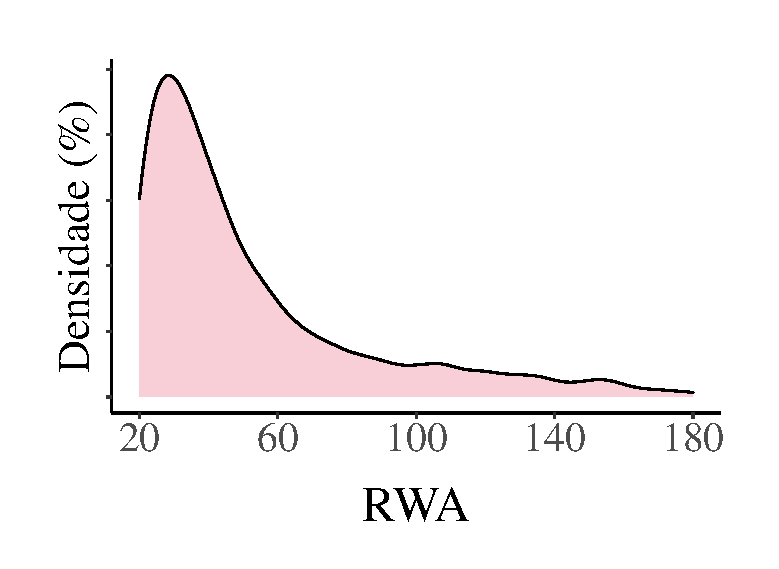
\includegraphics[width=1\linewidth]{figures/distribuicao_rwa}
		
		Fonte: \citeonline{open2016rwa}
	\end{minipage}
	\hspace{.05\linewidth}
	\begin{minipage}[b]{0.4\textwidth}
		\caption{Distribuição do Índice de Pós-Materialismo}
		\label{fig:pos_mat}
		\centering
		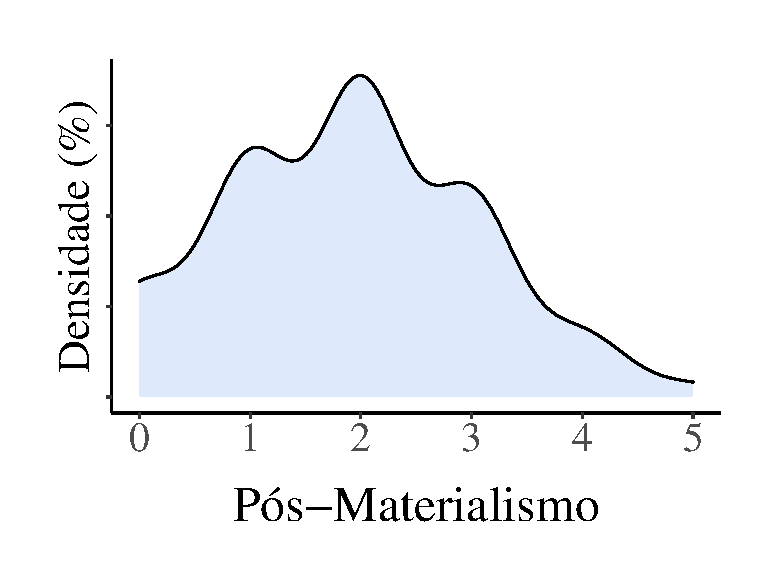
\includegraphics[width=1\linewidth]{figures/pos_materialism_index}
		
		Fonte: \citeonline{wvs2014wave}
	\end{minipage}
\end{figure}

Como efeito da sobreposição de elementos associados a confiança, tolerência e percepção de insegurança, o radicalismo ideológico associado ao RWA possui uma ocorrência esparça na população. Nas Figuras 1 e 2 é possível comparar a distribuição da escala com o Índice de Pós-Materialismo, proposto por \citeonline{inglehart2005modernization} e reconhecido como um indicador preciso de comportamentos liberais e pró-democráticos. Os dados sugerem que indivíduos com valores elevados para RWA estão longes do ponto mediano e, por isso, formam uma bolha atitudinal diferente do que observamos com indivíduos com baixos valores para Pós-Materialismo.

A existência de bolhas autoritárias na população tem efeitos significativos sobre a manutenção e replicação de movimentos radicais, os quais foram explorados em artigos sobre o tema. Além da maior imunidade em relação a formas distintas de pensamento -- lembre-se que o eleitor mediano e as propostas que visam-no estão distantes das faixas mais autoritárias -- essa parcela do eleitorado é facilmente mobilizável por \emph{outsiders} ou segmentos de representação dispostos a capturar suas intenções \cite{norris2017western, alexander2017myth}.  

De fato, em termos de dinâmica eleitoral, expera-se que a relação entre eleitores e representantes autoritários seja muito mais orgânica do que a interação convencional. Regimes autoritários podem angariar grande apoio popular, se uma parcela consistente da população percebe as restrição às liberdades como uma medida necessária contra ameaças e valida as fontes de informação do governo \cite{geddes1989sources, stein2013unraveling}. Portanto, é intutitivo concluir que a natureza da representação política para indivíduos autoritários é marcada por fortes traços delegativos.

\section{O discurso autoritário}

O discurso é um exercício de poder. É por meio da linguagem que registramos conhecimento, leis e regras de comportamento. Estes, por sua vez, compõem as principais categorias que humanos utilizam como referencial para interpretar o mundo ao seu redor. Por exemplo, se observamos alguém furar uma fila, julgamos sua atitude como justa ou oportunista, legal ou criminosa e moral ou anti-ética. Esses termos estão diretamente conectados a instituições sociais como o Estado e a Religião. 

Contudo, é importante ressaltar que, apesar dos grandes enunciados que constituem nossos guias de comportamento estarem ancorados na crença coletiva de sua validade, a capacidade de instituí-los está concentrada em poucos indivíduos \cite{foucault1969archeologie}. Ou seja, populações creditam legitimidade às suas leis e religiões, porém apenas uma pequena parte da nação é capaz de exercer influência direta no conteúdo de constituições e ritos.

A existência de um ranking social, que possui lugar de destaque para poucos e de subalternidade, para muitos, possui gênese anterior a civilização como conhecemos. As assimetrias que observamos nas relações sociais são fruto de um longo histórico de disputas e competição que acompanham a trajetória de sobrevivência de todas as espécies. Nessa dinâmica, a subserviência pode ou não ser conquistada por meio da força, mas sua manutenção se dá de maneira pacífica, na medida em que é naturalizada. 

Dentre as causas da hierarquia entre indivíduos, que funda a desigualdade observada na comunicação, a literatura aponta características individuais como determinantes significativos do desenvolvimento de dominância em grupos animais e humanos. Pesquisas documentam cor \cite{bakker1983determinants}, idade \cite{cote2000dominance, bohlin2001determinants}, peso corporal \cite{morgan2000predictors}, altura \cite{huang2002camera} e aparência \cite{lawson2010looking, lodge2013rationalizing} como alguns dos preditores da posição social de um indivíduo.    

Se por um lado características individuais explicam o surgimento da dominância, por outro, não são o único ingrediente do surgimento e estabilidade de cadeias de hierarquia que envolvem muitos integrantes. A disputa pelo lugar de dominância é mediada pela dinâmica interna dos grupos que compõem uma sociedade \cite{ridgeway1989dominance} e, em seguida, das relações entre os grupos \cite{chase1980social,chase2002individual}. Ou seja, a desigualdade é segmentada por clivagens formadas a partir de uma dinâmica complexa que envolvem aglutinações hierarquizadas de individúos em grupos que podem ser ordenados por status.  

Como argumentam \citeonline{sidanius2001social}, uma vez que grupos sociais são formados em torno de clivagens específicas -- por exemplo idade, gênero, clãs, nacionalidade, religião, cor e classe social -- seus integrantes reproduzem comportamento competitivo no qual buscam estabelecer superioridade. Nessa dinâmica, a formação de grupos dominantes e dominados estabelece a base da desigualdade, que consiste em uma super-atribuição de valores positivos aos dominantes e, de valores negativos, aos dominados. Dado que discursos refletem relações de dominância presentes na sociedade, expressões linguísticas do autoritarismo tendem a carregar traços valorativos presentes no seu conteúdo ideológico: a exaltação das figuras reconhecidas como autoridade e a depreciação de grupos minoritários de status social mais baixo. 

Isto posto, o autoritarismo pode ser lido como uma propriedade que emerge de sistemas sociais desiguais e hierarquizados, nos quais a dominância é reafirmada como narrativa política. Conforme argumentou-se na seção anterior, indivíduos autoritários apresentam maior propensão a expressão de preconceito e discriminação em geral. Ainda sobre o conteúdo de discursos autoritários, a literatura aponta a conexão entre autoritarismo e demonstração de hostilidade \cite{siegel1956relationship} e trabalhos que se dedicaram a investigar grupos políticos extremistas produziram resultados que sugerem que o dogmatismo político está correlacionado ao uso de discurso de ódio contra adversários e minorias \cite{gerstenfeld2003hate, ben2016hate}.  

O discurso autoritário apresenta ainda dimensões relevantes no que dizem respeito a sua forma e estilo. \citeonline{beauzamy2013discontinuities} argumentou que dois traços comuns ao discurso fascista no passado e no presente, são: i) o uso de argumentos elaborados com base em pseudo-ciência, teorias da conspiração, considerações mágicas e exegese religiosa e ii) uso de clichês e esteriótipos populares como metáforas em menções pejorativas a populações marginalizadas. Numa investigação similar, \citeonline{khany2014systemic} analisaram 20 discursos de personalidades históricas como Hitler, Stalin e Gadhafi. Como características comuns, apontaram a i) o majoritarismo e a massificação, ii) a defesa da incorruptibilidade do governo e iii) a manipulação das expectativas da opinião pública.

Em convergência com essa caracterização, \citeonline{smith1990symptomology} apresentou contribuição relevante para uma tipologia dos discursos autoritários analisando debates parlamentares acerca da ``proibição do fomento a homossexualidade'', que ocorreram entre as décadas de 80 e 90, nos EUA. Segundo a autora as falas autoritárias que emergiram sobre o tema apresentavam um traço marcante: a evocação de preconceitos e associações espúrias como método de enquadrar a discussão de forma desfavorável para a população gay. Em um dos exemplos dessa atitude, a menção à soropositividade como \emph{link} entre homossexualidade e problemas de saúde pública:

\begin{quote}
	A hegemonic interpretation of the AIDS phenomenon is, for example, actually a representation of radical difference, situated within a long tradition of similar representations of 'other' social elements. This AIDS discourse is linked genealogically to popular anxieties about various diseases, communist infiltration, immigrant populations, crime 'waves', drug 'crazes', etc. \cite{smith2015advances}
\end{quote}

A conexão entre soropositividade e homossexualidade é um caso típico do fenômeno cognitivo documentado como \emph{illusory correlation}, segundo o qual duas categorias de eventos são associadas sem que sua co-ocorrência estatística seja significativa. Além de uma inferência incorreta, capaz de estimular conclusões inadequadas, está na raiz do reforço de esteriótipos de raça, gênero e sexualidade que fazem parte do discurso autoritário. Quando indivíduos percebem maior frequência relativa de comportamentos rejeitados em um grupo, há uma tendência de identificá-los como atributo intrínseco ao grupo em questão, mesmo que a ocorrência absoluta de ``imposturas'' seja baixa \cite{sidanius2001social}.   

Além da frequente expressão de rejeição às populações identificadas como desviantes, discursos autoritários também envolvem constantes apelos a restauração da autoridade. Narrativas organicamente conectadas com o passado, que proclamam a restauração da ordem social e dos bons tempos que precederam o período atual tendem a ser instrumento de políticos autoritários para se colocarem como alternativas de crise \cite{pinto2004indoctrinating, mietzner2014indonesia}. 

Com isso, políticos autoritários as vezes se apresentam como alternativas radicais para condução de processos revolucionários ou de transição radical. Nesses cenários, discursos populistas que antagonizam as elites no poder com o ``verdadeiro povo'' são a principal estratégia eleitoral lideranças \cite{muller2017populism, levitsky2018democracies}. A proclamação de uma conexão íntima com a cultura, a tradição e os anseios da massa e o uso de forma verbal imperativa, autocentrada e reativa também são características marcantes de figuras autoritárias que buscam estabelecer uma nova hegemonia \cite{goldschlager1982towards, gounari2018authoritarianism, hunter2019bolsonaro}.

Tendo isso em mente, é importante considerar que, como agentes políticos que disputam eleições, o uso estratégico da fala é uma variante importante para compreender a forma e o conteúdo dos discursos de lideranças autoritárias em regimes democráticos. É especialmente em sistemas polarizados e com muitos partidos, em que a decisão do eleitorado tende a ser mais complexa, que características pessoais ganham relevância no debate público \cite{adams2011candidates,curini2015conditional}. Nesses contextos, antagonizar com o \emph{establishment} democrático e com as regras constitucionais em prol da imagem de líder que não vê barreiras para realizar seus ideais compõem uma plataforma tática de campanha.   

Em síntese, o discurso autoritário é marcado por forte traço de polarização entre autoridades e indivíduos desviantes. Seja por referência direta ou indireta, às autoridades são atribuídas fortuna moral e, aos desviantes, todo o mal experienciado pelos "verdadeiros cidadãos". De modo a cristalizar valores e dogmas, políticos autoritários frequentemente apelam para falas majoritaristas que relembram o passado de maneira nostálgica e acentuam as ameaças do presente. Como solução, apresentam-se em falas imperativas e hierarquizadas como guias para retomada da ordem e segurança. 

\section{Expectativas da Literatura}

Além de identificar características quanto a forma e conteúdo das narrativas autoritárias, investigações sobre o tema também reúnem um conjunto de fatores associados ao autoritarismo e aos grupos que apresentam maior prevalência de manifestá-lo. \citeonline{adorno1950authoritarian}, em seu trabalho seminal, apontou a rigidez e uso de violência da educação das crianças como um determinante central no desenvolvimento de atitudes autoritárias. Evidências coletadas posteriormente sugerem que a agressividade imposta na socialização primária eleva as taxas basais de estresse dos indivíduos e naturaliza a coerção como instrumento de negociação nas interações sociais \cite{hopf1993authoritarians, van2009authoritarianism}.

Apesar das críticas direcionadas a Adorno devido a sua interpretação do autoritarismo enquanto patologia psicológica, a família certamente permanece como preditor relevante para personalidade autoritária. Pais transmitem seus valores aos filhos, especialmente quando esses valores envolvem posições radicais e restritivas. Além do efeito geracional direto, a composição familiar é responsável por favorecer a formação de atitudes autoritárias por meio de \emph{in-group favoritism} \cite{lewis2014common, altemeyer2006authoritarians}. O familismo, desenvolvido a partir de conexões familiares profundas, pode ser responsável por limitar o convívio com comportamentos diversos e envolver os mais jovens em posicionamentos conservadores.

Outro vetor de força contrário a formação de uma mentalidade aberta e tolerante reside na religião. O fundamentalismo religioso oferece, em grande medida, precondições para adesão à narrativa autoritária: a crença em uma verdade eterna sobre a vida e o destino da humanidade, que depende do embate entre as forças do bem e do mal e da manutenção de práticas e tradições estabelecidas no passado \cite{rokeach1956political,rokeach1960open}. Como evidência desse fenômeno, a literatura encontra associação negativa entre intensidade da adesão à um sistema religioso e atitudes anti-democráticas e intolerantes \cite{pereira2001sistemas,pereira2004sistemas,fuks2012atitudes}. Como efeito, são as congregações religiosas mais radicais que constituem as parcelas mais fiéis do eleitorado de políticos autoritários \cite{mudde2013exclusionary, betz2016against}.

A insegurança também integra o universo de covariáveis do autoritarismo. Os efeitos do RWA sobre a manifestação de preconceito e violência tendem a apresentar maior magnitude em contextos de maior ameaça objetiva ou medo de vitimização. Ataques terroristas impulsionam a manifestação de RWA e, além disso, atuam como moderadores do impacto do autoritarismo sobre aceitação do uso de tortura em guerras \cite{linden2018terror}. Outros trabalhos encontraram resultados similares tomando o apoio à medidas de vigilância e restrição da liberdade como variável dependente \cite{cohrs2005effects}. Estudos experimentais que manipularam a percepção de ameaça no mundo também encontram evidências de que RWA é função da avaliação do risco e da insegurança de um indivíduo \cite{duckitt2003impact,sibley2007effects}.

A conexão entre violência e valores autoritários é corroborada ainda pela literatura que mensura os efeitos da violência sobre comportamento prossocial. Resultados de \emph{surveys} aplicados pré e pós guerras civis apontam que o conflito é uma fonte exógena de cooperação intragrupal e rivalidade intergrupal  \cite{bauer2016can,bauer2018trusting}. Investigações sobre as consequências dos homicídios cometidos pelos carteis de droga no México, identificaram efeitos heterogêneos da violência na manifestação de solidariedade com as vítimas: entre aqueles que tiveram parentes assassinados, a associação é positiva, já entre aqueles que não tiveram parente assassinados, negativa \cite{schedler2014collapse,schedler2016criminal}.

Além de componentes socioculturais, fatores econômicos também estão correlacionados ao RWA. A literatura reúne evidências de que o desenvolvimento exerce efeitos profundos sobre a cultura política das sociedades. Durante o processo de modernização, conflitos redistributivos são amenizados por meio da elevação da renda média e as populações experienciam a formação de capital humano, que permite a construção de regras sociais mais tolerantes, seculares e individualistas \cite{sullivan1999psychological, inglehart2005modernization}. Nessa dinâmica, a amenização da insegurança existencial favorece uma solução cooperativa para os problemas coletivos e, portanto, aumentam o apoio popular à democracia.

A relação entre economia e autoritarismo também se faz perceber a partir dos segmentos ocupacionais do mercado de trabalho. Mesmo em países que passaram por uma trajetória consistente de aumento da produtividade absoluta ao longos das últimas décadas, populações rurais absorveram poucos benefícios desse processo e perderam renda relativa. Como resultado, evidências apontam que o campo, em geral, constitui um cinturão de votos em favor de lideranças autoritárias, em grande medida por concentrarem maiores níveis de insegurança existencial \cite{ballard2017economic, norris2019cultural, mamonova2019populism, berlet2019rural,mamonova2019understanding}. Além disso, no levantamento realizado pelo \citeonline{fbsp2017medo}, foram nos municípios de menor porte e nas regiões mais rurais do Brasil que se concentraram as maiores médias de autoritarismo entre os entrevistados.

Como síntese dos achados, podem ser definidas 4 hipóteses sobre os fatores associados ao autoritarismo:

\begin{itemize}
	\item \textit{H1 : Indivíduos que possuem vínculos profundos com a família e relações estreitas com outros grupos tendem a apresentar maior propensão a manifestação de autoritarismo.}
	\item \textit{H2 : Fundamentalistas religiosos possuem precodições cognitivas que favorecem a adesão a valores autoritários.}
	\item \textit{H3 : Pessoas expostas a maior risco de vitimização e maior percepção de insegurança estão mais propensas a aderir da narrativa autoritária.}
	\item \textit{H4 : Àqueles que integram setores primários e economicamente sensíveis à choques externos tendem a incorporar atitudes autoritárias.}
\end{itemize} 


\chapter{Como classificar Agentes Autoritários?}\label{metodologia}

\section{As estratégias convencionais}

Conforme foi apresentado na seção \emph{Autoritarismo na política}, no capítulo 2, diversos trabalhos em Ciência Política se dedicaram a identificar causas e efeitos de políticos autoritários em regimes democráticos. Para isso, utilizam-se de um conjunto de estratégias metodológicas para classificar um agente autoritário. Nesse capítulo, abordará-se os principais critérios de classificação da literatura: a Avaliação de Especialista, Análise de Movimento Político, Survey com Elites. Por fim será discutido o uso de Análise Automatizada de Conteúdo como técnica de extração de variáveis atitudinais a partir de dados textuais.

\subsection{Avaliação de Especialista}

A primeira e mais popular forma de classificação baseia-se em estudos de caso de lideranças políticas, nos quais suas atitudes e comportamentos são observados a partir de pronunciamentos, discursos e presença na mídia. A partir daí, são analisados holísticamente, tomando como base um referencial teórico, e, então, são identificados ou não como autoritários.

Alguns dos exemplos dessa abordagem podem ser encontrados nos trabalhos de \citeonline{seligson2003democracies}, \citeonline{seligson2005feeding}, \citeonline{weyland2013latin} e \citeonline{levitsky2018democracies}. Em cada um deles, as autoras e os autores identificam características nas lideranças políticas -- em geral chefes do executivo -- que sugerem comportamento anti-democrático. Em algum dos casos, como o de Chavez, na Venezuela, e do General Hugo Banzer, na Bolívia, atos realizados após o início dos seus governos também fazem parte do escopo de análise.

Entre as vantagens desse modelo de classificação, a precisão certamente é a principal delas. Construindo uma narrativa com tantos elementos, a credibilidade das suas conclusões é elevada. Pesquisas que optam por realizarem estudo de casos de líderes costumam oferecer um conjunto rico e convincente de evidências para seus resultados.

Apesar da precisão na identificação, a abordagem baseada na análise de especialistas apresenta grandes limitações. Como trata-se de uma extensa coleta de informações sobre um agente político -- não raramente realizada de forma não sistemática -- a capacidade de replicabilidade dessas pesquisas é baixa e sua abrangência é limitada. Como recursos de pesquisa são limitados, líderes autoritários tendem a ganhar espaço nessas investigações acadêmicas apenas após ascenção para lugares de poder nos quais já representam risco para o regime demcorático.

\subsection{Análise de Movimento Político}

Nas investigações da dinâmica eleitoral de movimentos autoritários em regimes democráticos, partidos políticos frequentemente são tomados como unidade de análise, porém movimentos sociais também integram essas análises \cite{caiani2017radical}. Como efeito, a literatura conta com um extenso histórico de pesquisas e registros que identificam a evolução desses partidos e grupos organizados ao longo da história recente, tanto no que diz respeito a desempenho como radicalização \cite{norris2005radical, mudde2009populist, caiani2017radical, mudde2016introduction, mudde2017ideational}. 

Como critério de clasificação de partidos autoritários, a Análise de Agenda Partidária baseia-se na ideologia expressa diretamente pelos partidos, em manifestos e programas de governo, na percepção do eleitorado da sua posição no espectro político, e das suas raízes históricas \cite{mudde2000ideology}. Frequentemente \emph{surveis} com o eleitorado também integram fonte de informação para o enquadramento em tipologias \cite{booth1984political, booth1994paths, macwilliams2016decides}. Como as unidades de análise estão presentes em pequeno número, ou são mensuradas de informa indireta, há, atualmente, uma grande cobertura no mapeamento realizado por pesquisadores independentes.

Um conjunto de trabalhos, que exemplifica essa abordagem, pode ser encontrada na literatura que trata de partidos políticos que herdaram, na sua fundação, recursos, conexões e ideologia dos governos autoritários que precederam as transições democráticas na América Latina \cite{loxton2015authoritarian, loxton2014authoritarian, lyons2016victorious, loxton2015authoritarian} e Europa Central \cite{grzymala2006authoritarian}. 

Nessas pesquisas, a construção de uma imagem de campanha baseada em uma extensa lista de referências aos signos militares, além forte conexão dos programas de governo com plataformas securitárias e anti-comunistas, compõem o critério de demarcação. Contudo, como esclarece \citeonline{mudde2000ideology}, investigar o fenômeno do autoritarismo, a partir de uma definição ideológica, possui uma limitação no que diz respeito a falácia ecológica:

\begin{samepage}
	\begin{quote}
		Although party ideology is said to be the most important criterion for classification, it is used only in an indirect way, i.e. through the eyes of the party itself (party name) or of the voters. \cite{mudde2000ideology}
	\end{quote}
\end{samepage}

Se por um lado é possível construir uma medida com grande cobertura e relativa precisão -- apesar discordâncias na classificação serem tema de discussões recentes da literatura \cite{glasius2018authoritarianism, mudde2016introduction} -- por outro há uma limitação no que diz respeito a profundidade das inferências baseadas em agentes políticos agregados.

\vspace{2cm}

\subsection{Survey com Elites}

A utilização de dados fruto de questionários aplicados a elites está presente no histórico de produções em Ciência Política\cite{hoffmann2007methods, andreadis2017elite}. Em consonância com a convergência recente da literatura para apontar papel preponderante das elites na formação da opinião pública \cite{zaller1992nature, gabel2007estimating, achen2017democracy}, essa abordagem é capaz de identificar o núcleo dos principais agentes de constuição e fomento de ideologias políticas.

A literatura que trata sobre populismo é um dos exemplos recentes de uso da técnica. Trabalhos como o de \citeonline{stavrakakis2017new} e \citeonline{andreadis2017european} dedicaram-se a utilizar respostas de \emph{surveis} aplicados a parlamentares para operacionalizar critérios de classificação de partidos populistas e mensurar a organicidade do vínculo entre representantes e eleitorado populista. Além disso, \citeonline{stevens2006authoritarian} dedicaram-se a identificar componentes da dinâmica autoritária entre elites políticas e civis -- no caso, a percepção de ameça e o apoio a soluções anti-democráticas.

Como argumenta \citeonline{ruth2015measuring}, a ferramenta de \emph{survey} permite a coleta de dados atitudinais de um universo maior de indivíduos que ocupam lugar de poder em governos. Parlamentares compõem uma peça importante em governos e na formação da opinião pública, porém permanecem inexplorados pela literatura. Devido às limitações das técnicas de análise de discurso, estudos de caso e entrevistas com eleitores em i) produzir resultados para grande número de casos ou ii) medir com precisão a ideologia política das elites políticas, uma parte importante da dinâmica populista permanece desconhecida. 

A posição de \citeonline{ruth2015measuring} pode ser facilmente estendida para o campo de estudos sobre autoritarismo. As técnicas revisadas ao longo desse cápitulo possuem limitações semelhantes às tratadas pelo autor e, consequentemente, as conclusões no que diz respeito a lacunas no conhecimento sobre autoritarismo entre parlamentares permanecem válidas. 

Todavia, \emph{survey} com elites possuem graves limitações. Um dos grandes impeditivos de sua execução é o acesso restrito a população de entrevistados. Como consequência, a periodicidade de bases de dados de atitudes políticas de parlamentares costuma ser baixa. Mesmo em iniciativas como o \emph{Comparative Candidate Survey} (CCS), que reune dados de questionários aplicados a candidatos e políticos em exercício de diversos países, possuem itens limitados no que diz respeito a mensuração da indicadores da personalidade autoritária. 

Como consequência das limitações, foram identificados apenas dois trabalhos nos quais autoritarismo foi mensurado direta ou indiretamente entre parlamentares por meio de \emph{survey} -- \citeonline{stevens2006authoritarian} e \citeonline{joly2018personality} são os únicos representantes da abordagem encontrados na revisão bibliográfica dessa dissertação. 


\section{Análise Automatizada de Conteúdo}

Diante das limitações das abordagens anteriores, estratégias metodológicas que fazem uso de artefatos computacionais para otimizar processos de classificação têm se apresentado como uma solução para identificação em larga escala de atitudes e comportamentos de agentes políticos. Em particular, a literatura em Ciência Política que faz uso de Análise Automatizada de Conteúdo tem expandido seu escopo para ganhar aplicações em i) extração de informação sobre etnicidade a partir de nome \cite{roberts2016introduction}, ii) identificação de saliência temática em discursos de parlamentares \cite{batista2016mensurando, moreira2016palavra}, iii) construção de variáveis baseadas em componentes textuais \cite{curini2015conditional} e iv) extração de posicionamento ideológico implícito \cite{slapin2008scaling, ceron2016first}.

Os principais trabalhos de referência para classificação de parlamentares baseado em discursos concentram-se no campo de estudos sobre populismo. A partir de técnicas de codificiação baseadas em dicionário de termos, algoritmos de foram capazes de replicar, com relativa precisão e elevada escalabilidade, a classificação realizada por codificadores individuais de discursos populistas \cite{pauwels2011measuring, rooduijn2011measuring, oliver2016rise}. De forma similar, outras investigações utilizaram processamento de linguagem natural para automatização de partes do processo de identificação, como o reconhecimento de entidades associadas a adjetivos populistas \cite{kyle2018populists} e detecção de \emph{triplets} -- tríades compostas por sujeito, verbo e predicado \cite{aslanidis2018measuring}.

Para além da classificação de atributos atitudinais, algoritmos de aprendizado de máquina também têm sido capazes de modelar fenômenos psicológicos complexos como discurso de ódio \cite{davidson2017automated, zampieri2019predicting}, hostilidade \cite{hopp2017does, vargo2017socioeconomic, liu2018forecasting}, agressividade \cite{orasan2018aggressive, sahay2018detecting, nikhil2018lstms} e depressão \cite{mowery2016identifying, chekroud2016cross, orabi2018deep}. Esses resultados sugerem que há grande extensibilidade das aplicações, inclusive no que diz respeito a \emph{features} psicossocionais complexas, dentre elas, a personalidade autoritária.

Outra vantagem das ténicas de análise automatizada de conteúdo são sua grande versatilidade em termos de fontes e unidades de análise. A literatura angaria grande número de aplicações em \emph{big data} provenientes de Redes Sociais, \emph{blogs}, documentos oficiais e, no que diz respeito a Ciência Política, discursos, pronunciamentos e manifestos partidários \cite{grimmer2013text, wilkerson2017large, gentzkow2019text}. A escrita registra boa parte da atividade de agentes políticos, tanto dentro como fora do plenário. Uma vez que a comunicação é uma das principais formas de exercício de uma mandato e meio orgânico de \emph{accountability}, espera-se grande potencialidade dessa abordagem.

Todavia, algumas ressalvas importantes quanto a natureza dos modelos estatísticos de texto precisam ser salientadas. \citeonline{grimmer2013text} apresentou os \emph{4 Princípios da Análise Quantitativa de Texto}, são eles:

\begin{itemize}
	\item All quantitative models of language are wrong–but some are useful.
	\item Quantitative methods for text amplify resources and augment humans.
	\item There is no globally best method for automated text analysis.
	\item Validate, Validate, Validate.
\end{itemize}

Os tópicos sintetizam as maiores dificuldades da literatura que consome as novas técnicas de processamento de texto. Primeiramente, há grande perda de informação do valor semântico das palavras e frases quando elas são transformadas em dados de entrada em modelo estatístico. O sarcamo, por exemplo, é um recursos liguístico frequentemente utilizado para acentuar negativas, porém é elemento relativamente subidentificado por algoritmos de análise de conteúdo \cite{maynard2014cares}. Além disso, modelos de análise automatizada de conteúdo são significativamente sensíveis aos dados que recebem como \emph{input}. Amostras diferentes são capazes de produzir resultados significativamente distintos, mesmo que compartilhem mesma fonte.  

No que diz respeito ao desempenho e validação dos métodos, em artigo de \citeonline{dacrema2019we}, os autores abordaram o estado da arte dos algoritmos de recomendação. De 18 algoritmos considerados como representativos da literatura, apenas 7 foram capazes de ser replicadas de maneira apropriada e, desses, 6 apresentaram performance na revisão inferior a alternativas clássicas. Além de questionar os avanços gerados por implementações mais sofisticadas, o trabalho foi capaz de revelar graves limitações na reprodutibilidade e consistência no desempenho de técnicas de apredizado de máquina como um todo.  

Retomando o problema de pesquisa o qual esta dissertação busca resolver, de forma geral, avalia-se que o universo de \emph{Text as Data} apresenta uma saída consistente para a classificação de políticos autoritários. O potencial para processamento de grandes bancos de dados, com a possibilidade de modelar características individuais complexas, permite uma abordagem abrangente das atitudes de atores políticos cujo ofício implica no exercício da oratória.

Conforme argumentou-se no Capítulo 2, para lideranças autoritárias, discursos são ferramentas de mobilização do seu eleitorado cativo. Nas democracias contemporâneas, é por meio da fala, carregada de traços marcantes, que estes agentes políticos sedimentam e usufruem da dominância que estabelecem. A literatura converge para apontar que indivíduos dominantes tendem a utilizar mais tempo de fala e maior eloquência em seus discursos. Portanto espera-se que um parlamentar autoritário utilize com maior frequência seu espaço no plenário e, com isso, forneça dados suficientes para sua identificação e minimizar a ocorrência de falsos negativos. Autoritários silenciosos são tão raros quanto democratas no comando de ditaduras. 

\chapter{Propondo uma nova Mensuração}

\section{Introdução}

O uso de Análise Automatizada de Conteúdo para extração de variáveis atitudinais de dados textuais possui limitações. A principal razão delas está no fato de que as informações tomadas na modelagem advém de uma endógena de manifestação de crenças e preferências: o discurso. Todavia, essa estratégia apresenta-se como uma solução metodológica eficiente para construção de uma medida alternativa de autoritarismo capaz de ser implementada em larga escala, atualizada com frequência e adaptável para diversos canais de comunicação, inclusive Mídias e Redes Sociais. Nos parágrafos a seguir, serão detalhados os passos e pressupostos dessa empreitada.

Como ponto de partida, é importante conceituar a dinâmica de manifestação do autoritarismo por meio de discursos. Na Figura 3 é possível visualizar uma diagrama de um discurso político, que é formado por 3 elementos fundamentais: Entidades, objetos textuais aos quais se atribui sentido e significado; Atributos, que são os elementos que adicionam qualidades e significância às Entidade; e Temas, porções do discurso que agregam múltiplas Entidades e Atributos em torno de um conjunto de significados maior. Esses 3 elementos são dispostos pelo orador ao longo do seu tempo de fala e, como consequência, sentenças apresentam-se temporalmente correlacionadas. Ou seja, o que foi dito antes afeta o significado do que é dito depois.

A composição de Entidades, qualificadas por Atributos e agregadas em Temas, especifica a forma pela qual agentes dispõem suas atitudes políticas na forma de um discurso. Como efeito da intencionalidade do orador, Entidades, como `governo', `elite' e `povo', por exemplo, são tomadas como objeto de fala sobre o tema `crise atual', e é por meio dos Atributos associados às Entidades e ao Tema que consegue-se apreender o posicionamento latente do agente político em relação as Entidades mencionadas. Se os Atributos associados a uma Entidade são depreciativos ou se ela foi mencionada no contexto de um Tema que carrega uma carga de sentimentos negativo é intuitivo inferir que trata-se de um objeto de oposição para orador.

\begin{figure}[h]
	\caption{Diagrama do Discurso Político}
	\label{fig:discourse_representation}
	\centering
	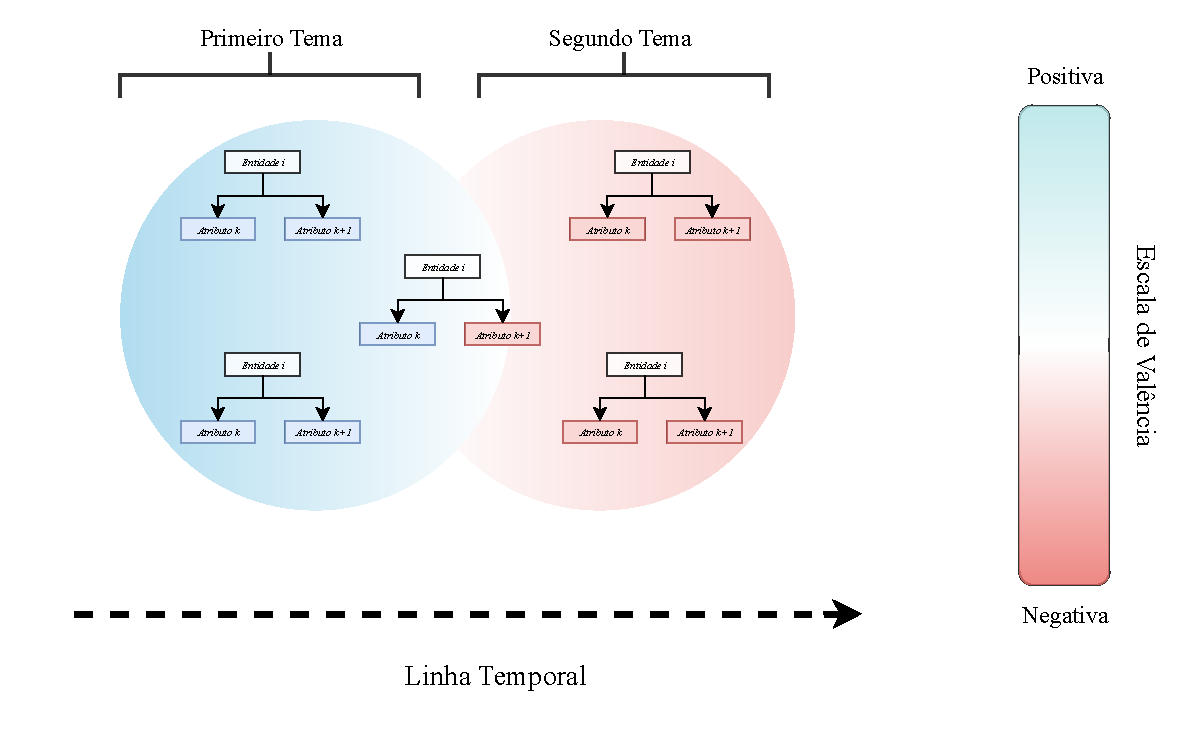
\includegraphics[width=1\linewidth]{figures/diagrama_discurso_autoritario}
	Fonte: elaboração do autor
\end{figure}

Ainda sobre o exemplo da Figura 3, as Entidades mencionadas no início do discurso tanto recebem atributos positivos como compartilham de uma atmosférica temática de Valência\footnote{Valência, nesse sentido, significa a escala de polaridade adjacente a um texto, o quão positivo ou negativo é a intenção expressa em relação a uma Entidade. O termo foi popularizado pelos trabalhos no campo da Análise de Sentimentos, que buscam modelar a polaridade de sentenças e de tópicos.} mais positiva. No outro extremo, as Entidades mencionadas ao final do discurso possuem o inverso dessas características -- Atributos e Tema e negativos. Portanto, pode-se inferir que, no escopo de Entidades do orador, seu posicionamento variou da simpatia manifesta no início da fala até a rejeição, ao final. Essa dinâmica discursiva remete ao caráter hierárquico da estrutura textual, na qual termos são unidades básicas da linguagem, sentenças concatenam sentido no nível local, e temas consolidam grandes conjuntos de expressão.    

Um exemplo prático dessa dinâmica está presente nas contribuições de \citeonline{smith1990symptomology}. Nas falas de parlamentares analisadas pela autora, a expressão de rejeição à minorias apresentou dois modos típicos: i) a atribuição direta de características negativas e ii) o estabelecimento de uma correlação ilusória a partir da menção de Entidades em Temas carregados de polaridade negativa -- como crime, entorpecentes e problemas de incivilidade. Do ponto de vista dos ouvintes, um grupo social que compartilha um mesmo espaço semântico que elementos popularmente reprovados também é passível de estigma. De forma simétrica, a exaltação de Entidades associadas às autoridades se dá pelos mesmos mecanismos.

Além do uso de Atributos, a posição em relação a uma Entidade é fortemente marcada pela frequência em que é mencionada nas falas de um agente. A saliência temática demarca tanto clivagens políticas como espaços de embate, uma vez que, no contexto de recursos limitados, é o principal indicativo de quais são as questões prioritárias. A recorrência na menção de uma pauta ou maior investimento de tempo de fala em discursos nos quais é mencionada eleva a magnitude das opiniões mobilizadas em torno dela e é determinante da ideologia do orador.

É intuitivo assumir, ainda, que Entidades, Atributos e Temas são elementos que se combinam de forma complexa em discursos politizados com o propósito de expressar conteúdo ideológico. Ou seja, é possível utilizar informação da fala dos oradores para inferir posicionamentos latentes e, no caso deste trabalho, estimar seus níveis de RWA. Para isso, assume-se que a Valência expressa em relação a certas classes de Entidade pode ser traduzida em adesão à grupos dominantes -- polaridade positiva -- e rejeição à grupos dominados -- polaridade negativa.

\section{Definindo uma Tipologia de Entidades}

Uma vez que o discurso autoritário é composto por uma estrutura básica de atribuição de significado, segundo a qual autoridades e aos valores tradicionais são sobrevalorizados e grupos identificados como populações desviantes, subvalorizadas, uma tipologia que identifique Entidades associadas a cada uma dos grupos se faz necessária para identificar o nível de adesão à narrativa autoritária. No Quadro 1 é possível observar uma tipologia de Entidades baseada na escala original proposta por \citeonline{altemeyer2006authoritarians} e nas versões brasileiras das escalas de RWA e F, adaptadas respectivamente por \citeonline{vilanova2018adaptaccao} e \citeonline{de2018analises}. 

No Quadro 1, as divisões correspondem aos Componentes que Integram a Escala RWA, aos Valores que representam dimensões específicas nas quais cada componentes se manifesta e as Raízes que identificam elementos textuais associados a cada Valor. As Raízes são porções genéricas de palavras, sem prefixo, sufixos e conjugações, e no quadro elas identificam as principais Entidades que representativas de cada Valor. É partir desse mapeamento que é possível observar em quais falas uma gente político está se manifestando sobre cada um dos Valores Autoritários e, como consequência, mensurar seu posicionamento em relação a eles.

Para elaboração da Tipologia foram realizados dois esforços: o primeiro envolve a identificação dos Valores Autoritários e o segundo, da Raízes textuais representativas de cada Valor. Para isso foram analisados os questionários originais, propostos por \citeonline{altemeyer1981right} e \citeonline{adorno1950authoritarian}, e as adaptações das escalas para o contexto brasileiro, realizada por \citeonline{vilanova2018adaptaccao} e \citeonline{de2018analises}. Ao longo de todas as perguntas dos questionários, além das dos 3 Componentes fundamentais do autoritarismo foram identificados 8 subcomponentes -- ao qual denominou-se de Valores -- que dizem respeito a elementos específicos da manifestação de cada componente. Já para definição das Raízes, tomou-se como base o trabalho realizado por \citeonline{moreira2016palavra}, que mapeou os tópicos constitutivos do debate político brasileiro a partir do resultado de \textit{expressed agenda model} e dados textuais de pronunciamento parlamentares. O mapeamento das Raízes foi finalizado a partir da consulta de sinônimos de conjugações de alguns dos termos. 

\begin{center}
	Quadro 1 - Tipologia de Entidades
	
	\vspace{0.4cm}
	
	\begin{tabular}{llc}
		\toprule
{Componente}								& {Valor} 					& {Raízes} \\ \midrule
\multirow{2}{*}{Submissão à Autoridade} 	& Ufanismo				& \textit{brasil}, \textit{patri}, \textit{nação}, \textit{herói} \\
& Radicalismo Religioso		& \textit{deus},\textit{igreja},\textit{evangelic},\textit{catolic},\textit{crist},\textit{crent} \\ \midrule
\multirow{3}{*}{Agressividade Autoritária} 	& Punitivismo 				& \textit{polic}, \textit{seguranc}, \textit{milit}, \textit{exercit}, \textit{forcas} \\
& Patriarcalismo	 		& \textit{famil}, \textit{tradic}, \textit{home} \\
& Rejeição à Diversidade	& \textit{negr},\textit{racial},\textit{homossex},\textit{lesb},\textit{human},\textit{indigen},\textit{mulh} \\ \midrule
\multirow{3}{*}{Convencionalismo} 			& Majoritarismo 			& \textit{povo}, \textit{nós}, \textit{cidad}\\
& Hierarquia				& \textit{autorid}, \textit{trabalh}, \textit{empreg}, \textit{banc}, \textit{financeir} \\
& Anti-cientificismo		& \textit{estud}, \textit{univers}, \textit{pesquis}, \textit{cienc}, \textit{cient}, \textit{tecno} \\ \bottomrule
	\end{tabular}
	
	\vspace{0.6cm}
	
	Fonte: elaboração do autor com dados de \citeonline{moreira2016palavra} 
\end{center}

No que diz respeito aos Valores que integram a Tipologia de Entidades, no contexto brasileiro, Ufanismo, Majoritarismo e Punitivismo são elementos centrais da narrativa que saúda o passado e propõem uma saída centralizadora e monotônica, que se utiliza do militarismo, para restauração. Entre os questionários originais e adaptados, estão presentes fortes referências a salvação do país por meio de punição mais rígidas e laços mais entreitos entre Estado e Sociedade Civil. Alguns dos exemplos extraídos das perguntas realizadas nos questionários são:

\begin{quote}
	1. Do jeito que as coisas estão indo nesse país, serão necessárias medidas severas para endireitar os meliantes, os criminosos e os pervertidos.
	
	2. A situação do nosso país está ficando tão séria que ações firmes seriam justificadas se eliminassem os desordeiros e nos levassem de volta ao nosso verdadeiro caminho.
	
	6. O que o nosso país realmente precisa é uma dose forte e dura de lei e ordem.
	
	29. Nosso país será melhor se obedecermos nossos líderes.
	
	34. Nosso país será melhor se mostrarmos respeito à autoridade.
	
	3. Não há nada pior do que uma pessoa que não sente profundo amor, gratidão e respeito por seus pais
	
	\cite{vilanova2018adaptaccao, de2018analises}
	
\end{quote}  

Além de aspectos políticos, também é possível observar uma dimensão associada a atitudes e comportamentos captada pelos valores de Radicalismo Religioso, Patriarcalismo e Rejeição à Diversidade. Cada um dispõe de um conjunto próprio de julgamentos que segmentam a população entre ``bons'' e ``maus'', oferecendo as bases para discriminação e intolerância contra grupos vulneráveis, minorias e indivíduos que questionam a autoridade e a tradição. É possível visualizar alguns desses elementos normativos a partir das afirmativas a seguir que integram os componentes para o calculo das escalas adaptadas por \citeonline{vilanova2018adaptaccao} e \citeonline{de2018analises}:
 
\begin{quote}
	
	15. As pessoas devem estar prontas para desafiar leis com as quais elas não concordam.
	
	
	18. As pessoas deveriam ter as suas próprias preferências sexuais, mesmo se isso torná-las diferentes do resto da sociedade.
	
	19. Não há nada de errado com sexo antes do casamento.
	
	21. As pessoas deveriam ter os seus próprios estilos de vida mesmo se isso torná-las diferentes do resto da sociedade.
	
	24. As leis de Deus sobre aborto, pornografia e casamento devem ser seguidas à risca antes que seja tarde demais.
	
	6. Todos devemos ter fé absoluta em um poder sobrenatural, cujas decisões devemos acatar.
	
	10. Os homossexuais são quase criminosos e deveriam receber um castigo severo.
	
	\cite{vilanova2018adaptaccao, de2018analises}
	
\end{quote}

Por fim, a Hierarquia e Anti-cientificismo selam um bloqueio triplo contra as principais fontes de contestação na sociedade: aqueles que não ocupam a posição de poder e aqueles que produzem novos conhecimentos. Autoritários tendem rejeitar contestações a suas crenças e apegam-se veementemente aos papeis sociais tradicionais, naturalizando a desigualdade. Buscando identificar esse tipo de disposição, os questionários incluem as afirmativas:
 
\begin{quote}
	
	16. Estudantes de colégios e universidades devem ser encorajados a desafiar, criticar e confrontar autoridades.
	
	13. A ciência tem o seu lugar, mas há muitas coisas importantes que a mente humana jamais poderá compreender.
	
	14. Os homens podem ser divididos  em duas classes definidas:  os fracos e os fortes.
	
	16. Pobreza é consequência da falta de vontade de querer trabalhar.
	
	\cite{vilanova2018adaptaccao, de2018analises}
	
\end{quote}

Como resultado da manifestação de adesão ou rejeição aos componentes do autoritarismo obtém-se uma Escala de Valores Autoritários, que varia entre 0 e 8 pontos -- dado que identificou-se 8 subcomponentes do RWA. A escala busca extrair dos discursos as informações obtidas por meio dos questionários, porém como tratam-se de manifestações endógenas de atitudes, é preciso considerar que a expressão de posicionamento ocorre de maneira direta -- a nível de sentença -- ou indireta -- a nível de tema. No primeiro caso, Atributos associados às Entidades identificam a opinião, já no segundo caso, é o contexto, formado pelo conjunto dos Atributos das Entidades mencionadas sob um Tema, que apresenta o a posição em relação ao Valor. 

\section{Definindo os Componentes de Mensuração}

A Equação 3.1 especifica a estimação de expressão direta. Dado um Valor $v$, que compõem uma das dimensões do RWA, a adesão de um agente político se expressa pela razão da diferença entre o número de sentenças positivas -- $Pos_v$ --  e o número de sentenças negativas -- $Neg_v$ -- que mencionam alguma das Raízes que compõem a tipologia de Entidades no Quadro 1 e o número de sentenças de sentimento mais frequente -- $Pos_v$ ou $Neg_v$.

\begin{equation}
\beta_v = 
\begin{cases}
\frac{Pos_v - Neg_v}{Pos_v}, & \text{se}\ Pos > Neg \\
\frac{Pos_v - Neg_v}{Neg_v}, & \text{caso contrário.}
\end{cases}
\end{equation}

A Equação 3.2 especifica a estimação de expressão indireta. Dado o contexto do Discurso $k$, em que Entidades que compõem uma das dimensões do RWA são mencionadas, a adesão indireta de um agente político se expressa pela razão da diferença entre o número de sentenças positivas -- $Pos_k$ --  e o número de sentenças negativas -- $Neg_k$ -- contidas no contexto e o número de sentenças de sentimento mais frequente -- $Pos_k$ ou $Neg_k$.

\begin{equation}
\gamma_k = 
\begin{cases}
\frac{Pos_k - Neg_k}{Pos_k}, & \text{se}\ Pos > Neg \\
\frac{Pos_k - Neg_k}{Neg_k}, & \text{caso contrário.}
\end{cases}
\end{equation}

As estimativas geradas pelas Equações 3.1 e 3.2 resultam em valores que pertencem ao intervalo $[-1, 1]$, em que quanto mais próximo de 1, maior a probabilidade de adesão a um dos Valores que compõem a escala de Valores Autoritários e, mais próximo de -1. menor a probabilidade de adesão. 

Por fim, o indicador final é composto pela soma ponderada das duas estimativas, especificada na Equação 3.3. A escala de adesão, representada por $\theta$, também varia no intervalo$[-1, 1]$. A Equação 3.4 representa a normalização do valor de $\theta$. Se um indivíduo possui resultante positiva, então apresenta algum nível de adesão ao valor autoritário e soma 1 ponto na Escala de Valores Autoritários. Como tratam-se de 8 Valores, a escala varia entre 0 -- rejeição de todos os Valores autoritários -- e 8 -- adesão à todos os valores autoritários.

\begin{equation}
\theta_{vk} = 0.75 * \beta_v +  0.25 * \gamma_k
\end{equation}

\begin{equation}
AuthVal_v = 
\begin{cases}
1, & \text{se}\ \theta_{vk} > 0 \\
0, & \text{caso contrário.}
\end{cases}
\end{equation}

Tomando um exemplo anedótico, para o valor de Punitivismo, um indivíduo que manifestou $\beta = 0.5$ -- portanto se inclinou diretamente ao Valor -- e $\gamma = -0.8$ -- inserindo a menção ao Valor em um contexto muito negativo -- apresenta $\theta = 0.175$ e, assim, recebe 1 ponto na escala de Valores Autoritários -- $AuthVal$. Para definir os pesos dos componentes de $\theta$, tomou-se como referência a literatura que trata de \emph{Social Desirability Bias}. Trabalhos que estimaram a subnotificação de compra de votos, xenofobia e racismo apresentaram resultados entre 20{\%} e 30{\%} \cite{rudmin1999norwegian,heerwig2009education,gonzalez2012vote}.

É necessário, contudo, lidar com um fator adicional. Como agentes políticos possuem agendas diferentes, é esperado que apenas uma parte dos oradores façam menção à todos os Valores da escala de Valores Autoritários, seja para manifestar adesão ou rejeição. Um parlamentar que possui pautas sanitárias como centro da sua representação, por exemplo, tende a se manifestar sobre questões punitivas com menor frequência. Como efeito, a escala apresenta viés de seleção e incorpora efeitos endógenos da saliência temática dos agentes políticos.

Como forma de aproximar a escala de Valores Autoritários de um indicador consistente de RWA, utilizou-se inferência bayesiana. Nesse sentido, a estimativa de RWA de um agente político é composta por uma porção de informação a priori, que envolve o que sabe-se sobre a distribuição de RWA na população, e uma porção de informação definida pela verossimilhança, que obtem-se a partir dos dados, decomposta pela escala de Valores Autoritários. 

Como informação a priori, assume-se que o RWA entre agentes políticos segue uma distribuição Poisson, tal como sugerem os dados coletados a partir de respostas para questionário original, como na Figura 1. Uma vez que foram delimitados 8 conjuntos de Valores, a distribuição pertence ao intervalo $[0, 8]$, de parâmetro $\lambda = 1.62$\footnote{O parâmetro $\lambda$ foi estimado a patir dos microdados de \citeonline{open2016rwa}. Para isso, tomou-se a média da escala de RWA dos respondentes que levaram até o quantil 95 de tempo para responder o questionário e que cometaram no máximo até 2 erros, de 16, nas questões de validação.}. Para inferir uma média de RWA para a população, basta calcular a esperança da distribuição ao longo de todo o intervalo, representada pela área A na Figura 4.

\begin{figure}[!htb]
	\caption{Distribuição Priori e Posteriori RWA}
	\centering
	\begin{minipage}[b]{0.4\textwidth}
		\textbf{Priori}
		\label{fig:rwa_area_total}
		\centering
		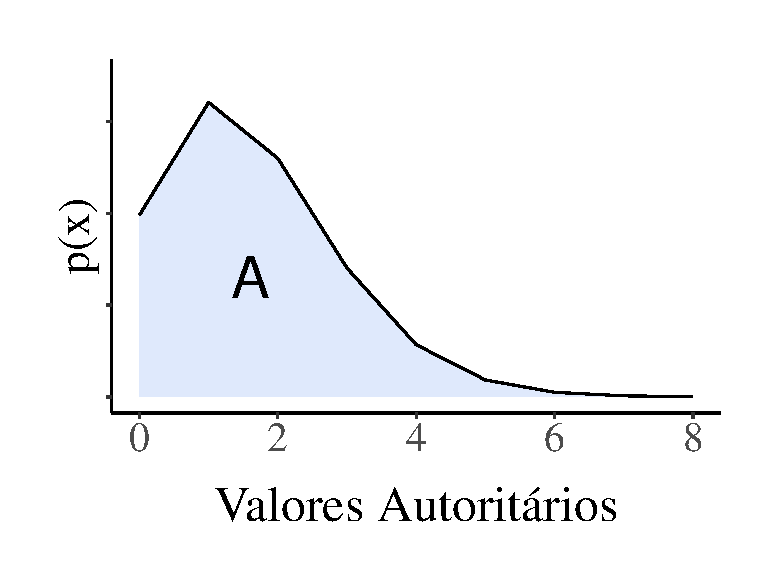
\includegraphics[width=1\linewidth]{figures/area_total_rwa}
			\end{minipage}
\\
	\hspace{.05\linewidth}
	\begin{minipage}[b]{0.4\textwidth}
		\textbf{Posteriori}
		\label{fig:rwa_area_min}
		\centering
		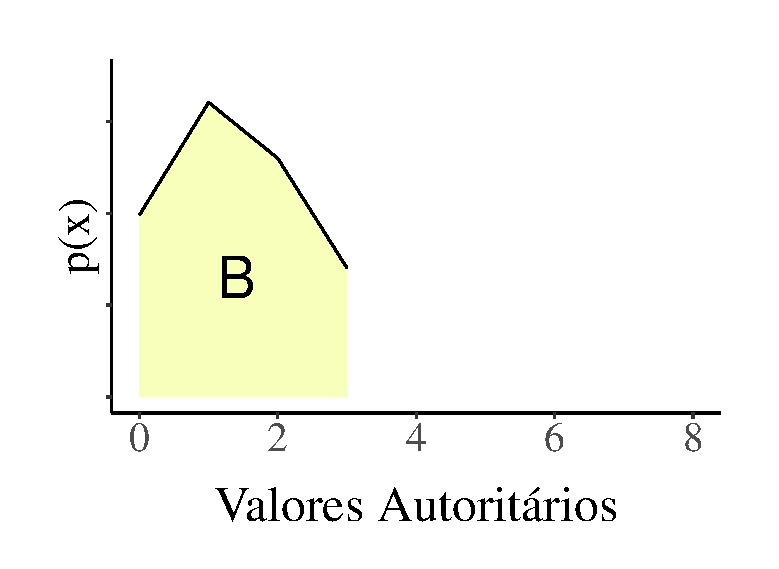
\includegraphics[width=1\linewidth]{figures/area_parcial_min_rwa}
		
	\end{minipage}
	\hspace{.05\linewidth}
\begin{minipage}[b]{0.4\textwidth}
	\textbf{Posteriori}
	\label{fig:rwa_area_max}
	\centering
	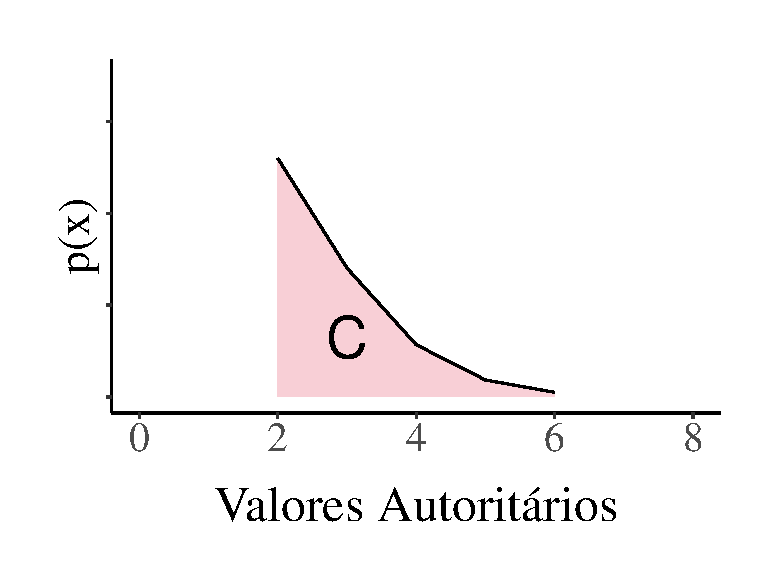
\includegraphics[width=1\linewidth]{figures/area_parcial_max_rwa}
	
\end{minipage}

Fonte: elaboração do autor
\end{figure}

Como ponto de partida, é intuitivo atribuir o valor médio a um agente político qualquer. Porém, na medida em que adquirimos mais informação, mensurando a escala de Valores Autoritários, é possível introduzir condicionais no cálculo da esperança, restringindo o espaço de eventos e conseguindo alcançar um valor médio que converge para um ponto mais preciso. 

Na Figura 4, na área B, também é possível visualizar o polígono resultante de um indivíduo que se manifestou sobre 5 dos 8 Valores e rejeitou todos. Como efeito, dois cenários extremos são possíveis, caso se manifestasse sobre os outros 3 Valores: rejeitar todos ou aderir a todos. Com isso, a aŕea que corresponde o espaço de eventos restringe ao polígono formado pela distribuição no intervalo $[0, 3]$. Já na área C, é possível visualizar a representação de um indivíduo que se manifestou sobre 4 Valores, aderiu a 2 deles e rejeitou outros 2. Nesse caso, os cenários extremos são: rejeitar os outros 4 e aderir a todos eles. Assim, o RWA estimado se retringe a esperança da distribuição no intervalo $[2, 6]$. Comparativamente, o valor de RWA estimado para os casos A, B e C são, respectivamente, 1.62, 1.37 e 2.68.

Alguns detaques importantes nos procedimentos de estimação são que a distribuição a priori, especificada na Equação 3.5 e visível na distribuição da área A, na Figura 4 resguarda os pressupostos de uma distribuição de probabilidade. Para que os polígonos gerados a partir da restrição de intervalos, como no caso das áreas B e C da Figura 4, contudo, é necessário atualizar os valores da variável aletória para que a integral da função de probabilidade resulte em 1, conforme especifica a função composta na Equação 3.6. 

A inclusão de num novo componente no denominador, que consiste na soma das probabilidades do valores que compõem o intervalo $[L, U]$, tem como efeito normalizar as probabilidades no polígono. Ou seja, a escala de Valores Autoritários entrega os parâmetros de \emph{upper bound} e \emph{lower bound}, utilizados para definir o espaço de eventos. Por fim, a Equação 3.7 especifica o cálculo da esperança da distribuição que tem como resultante o valor estimado de RWA e a Equação 3.8, a variância da estimativa. 
     

\begin{equation}
f(x) = \frac{\mathsf{e^{-\lambda}} \,\lambda^{x}}{x\,!}
\end{equation}

\begin{equation}
g \circ f(x,\, L, \,U) =\frac{\mathsf{e^{-\lambda}} \,\lambda^{x}}{x\,! \, \displaystyle\sum_{k = L}^{U} f(k)}
\end{equation}

\begin{equation} \label{eq1}
\begin{split}
\widehat{rwa} & = E(x) \\
E(x|L, U) & = \int_{L}^{U} g \circ f(x, L, U) \,x \,dx
\end{split}
\end{equation}

\begin{equation}
\begin{split}
\sigma^{2} & = E(x^{2}) \\
E(x^{2}|L, U) & = \int_{L}^{U} g \circ f(x, L, U) \,x^{2} \,dx
\end{split}
\end{equation}

É possível observar a proporcionalidade entre a quantidade de Valores Autoritários e o RWA estimado, porém os resultados obtidos por meio de atualização bayesiana apresentam correções contra subestimação e viés de seleção.

\section{Operacionalizando a Estimação dos Componentes}

Para estimarmos o valor de RWA de um agente político é necessário definir um método de mensuração da Valência das Sentenças associadas às Entidades. Conforme argumentou-se, a Valência é um componente que se expressa a nível de sentença e de contexto, manifestando a adesão e rejeição nas suas formas direta e indireta. É a partir do indicador de que uma sentença é positiva que pode-se calcular os parâmetros $\beta$ e $\gamma$ das Equações 3.1 e 3.2. E para definição do escopo do contexto, é necessário identificar a qual tópico ou tema a Entidade de interesse está inserida. Com as duas informações, é possível compor imagens como a Figura 3, que detalham a dinâmica discursiva de um discurso político.

Antes de detalhar a estratégia operacional é necessário caracterizar o uso da Valência como indicador de apoio e desaprovação. Para isso, é importante ressaltar que a validade de modelos baseados em dados textuais envolve a expectativa de que é possível estabelecer equivalência entre valores numéricos e emoções humanas. Além disso, todo modelo carrega um caráter de representação da realidade, que ganha precisão quanto mais for validada. Apesar de críticas que apontam que essas duas premissas são fortes demais para serem aceitas em pesquisas sobre comunicação política \cite{miguel2015vale}, a análise de valências têm se popularizado e conta com enorme respaudo acadêmico \cite{feres2016analise}.      

Como opção metodológica, adotou-se a Análise de Sentimentos, uma solução algorítmica para análise de textos, desenvolvida para extração e identificação de emoções, sentimentos e atitudes, altamente escalável. Ao longo das três últimas décadas, tem sido cada vez mais utilizada para a automatização no processamento de \emph{reviews} no mercado digital e extração de \emph{features} textuais de opinião pública. Quanto às premissas do modelo e o tipo de resposta que oferece, algoritmos dessa natureza partem do postulado de que toda sentença possui uma valência, ou seja, um posicionamento latente que pode ser tipificado em pró, contra ou neutro -- frequentemente assinalados com os valores -1,0 e 1 -- que representam as classes do \emph{target} na otimização do modelo \cite{serrano2015sentiment, mantyla2018evolution}.  

Uma das formas de calibrar o algoritmo consiste no uso de dicionários codificados, construídos a partir da classificação de termos e expressões que carregam carga semântica negativa ou positiva. Nesse sentido, alguns dos modelos propostos na literatura ancoram-se em artefatos produzidos no campo da linguística e psicologia para conectar palavras a sentimentos, inclusive com grande complexidade. Um desses exemplos é o PANAS-t, desenvolvido por  \citeonline{gonccalves2013panas}, que baseia-se na escala psicométrica PNAS, proposta por \citeonline{watson1988development} e posteriormente estendida por \citeonline{clark1994manual}. A escala, elaborada a partir de entrevistas nas quais respondentes descreviam como se sentiam em relação a certos eventos, identifica expressões associadas a afeição e rejeição. 

Anos antes, \citeonline{bollen2010determining} apresentaram um modelo baseado na escala POMS \cite{mcnair2003profile} que, partindo da mesma estratégia, identificava a valência de uma sentença a partir da frequencia relativa de suas palavras e suas correspondências como a tipologia estabelecida. Contudo, o estado da arte das estratégias baseadas em dicionários é ocupado por combinações de tipologias, uso de fontes mistas -- como \emph{emoticons} --  e processos generativos automatizados, como a interpolação da valência de uma palavra para seus sinônimos e tipificação baseada em coocorrência \cite{hogenboom2013exploiting, hutto2014vader, thelwall2014sentistrength, canuto2016exploiting}.

Uma alternativa às técnicas baseadas em dicionários são o modelos de \emph{Machine Learning} que tomam texto como \emph{features} na previsão de um \emph{target} que, nesse caso, é composto por classes de sentimentos\footnote{Do ponto de vista da implementação, as soluções mais simples prodecem da seguinte forma: 1) o texto é preprocessado, \emph{stopwords} e símbolos são removidos, 2) as palavras que compõem cada sentenção são divididas e as com menor frequência são retiradas 3) a partir de todas as palavras que compõem o banco de dados, sentenças são representadas por uma série de variáveis binárias que identificam a presença ou não de cada uma das palavras e 4) um modelo de regressão logística é treinado utilizando as variáveis binárias como variáveis independentes e o \emph{target}, como variável dependente. Soluções mais complexas envolvem métodos mais sofisticados de transformam das sentenças em variáveis numéricas -- como \emph{Word2Vec} -- e modelos mais adequados para lidar com multicolinearidade e otimização -- como \emph{Ensemble Learning}.}. O primeiro trabalho a adotar essa abordagem foi apresentado por \citeonline{pang2002thumbs} que, se utilizando de uma base de \emph{reviews} de produtos, tomou das \emph{n-grams} -- sequências contínuas de palavras -- das sentenças como \emph{inputs}. Atualmente, a literatura documenta modelos de elevado desempenho, que atingem grande precisão de classificação, mesmo como bases de treinamento rotuladas por não-especialistas \cite{howard2018universal, sun2019fine, yang2019xlnet}. Essa abordagem, contudo, implica em custos de elaboração e implementação significativamente caros, uma vez que imprescindem de codificação em larga escala e grande poder computacional para atingirem precisão satisfatória.

Para definição do modelo de classificação, relizou-se experimentos tomando os 4 principais dicionários léxicos de sentimentos para língua portuguesa: ReLi, LIWC, OpLexicon e SentiLex-PT. O ReLi concatena anotações de 1600 resenhas de 14 livros diferentes \cite{freitas2012vampiro, freitas2014sparkling} e foi transformado em léxico a partir do trabalho de \citeonline{freitas2013construccao} por meio da codificação de vocabulário afetivo. O LIWC é produto de uma investigação psicológica sobre a expressão de sentimentos de estados mentais por meio da linguagem que contou com aplicação extensa de questionários não-estruturados \cite{pennebaker1996cognitive, pennebaker1997linguistic}. Já o OpLexicon e SentiLex-PT se diferenciam das alternativas anteriores por utilizarem codificação automatizada na composição dos léxicos \cite{souza2011construction, carvalho2015sentilex}.

Quanto aos procedimentos realizados na etapa de preprocessamento do texto, as seguintes transformações são realizadas nas sentenças: i) eliminação de pontuação, símbolos e números; ii) remoção de \emph{stopwords} (artigos, preposições, conjunções ...); iii) conversão de todas as palavras da sentença para minúsculo. Vale ressaltar que as raízes das palavras não foram extraídas, uma vez que a flexão é relevante em classificações por dicionário léxico. Partindo da sentença preprocessada, para extração do sentimento, utilizou-se a regra de bolso adotada por \citeonline{gonccalves2013panas}, na qual as quantidades de termos positivos e negativos são relacionadas por meio da fórmula da Equação 3.9.

\begin{equation}
P(s) = 
\begin{cases}
\frac{\alpha_s - \beta_s}{\alpha_s}, & \text{se}\ \beta_s \leq \alpha_s \\
\frac{-1(\beta_s - \alpha_s)}{\beta_s}, & \text{se}\ \beta_s > \alpha_s
\end{cases}
\end{equation}

Sendo $P(s)$ a polaridade da sentença \emph{s}; $\alpha_s$ a quantidade de termos positivos na sentença e  $\beta_s$ a quantidade de termos negativos.

Como base de avaliação dos experimentos, utilizou-se um banco de dados, de elaboração própria, composto pelas setenças das 511 declarações de voto na sessão que discutiu a admissibilidade do \emph{impeachment} de Dilma Roussef. As sentenças foram codificadas manualmente em 3 categorias de valência: negativas, neutras e positivas. Uma vez que a sessão contou com grande audiência, num momento de intensas manifestações civis no país, as falas dos parlamentares manifestaram-se em um microcosmos de afetos políticos. Com isso, constitui-se um cenário ideal para mensurar a precisão de métodos de classificação de sentimentos.   

Para construção dos modelos, utilizou-se como referência o trabalho de \citeonline{machado2018creating}, os quais propõem estratégias de otimização no uso de dicionário léxicos em problemas de classificação\footnote{\citeonline{machado2018creating} definem estratégias que implicam em ganhos significativos de desempenho na classificação. A primeira delas consiste no uso de advérbios de negação como identificadores de pontos de inversão da valência de um atributo. Nos exemplos ``\textit{Não! Ele é honesto}'' e ``\textit{Ele \textbf{não} é honesto!}'', a referência a honestidade possui pesos opostos que são demarcados pela posição do termo 'não' na frase. Outra contribuição importante envolve os métodos de combinação de dicionários léxicos. Tanto nos experimentos realizados pelos autores como nos realizados neste trabalho, a opção por ordem de uso das predições implicou em resultados significativos diferentes.}. O desempenho de cada experimento pode ser visualizado na Tabela 1. As métricas de Precisão Ponderada e Recall Ponderado\footnote{As métricas de Precisão e Recall significam, respectivamente, a taxa de acertos do classificador -- positivos verdadeiros sobre positivos assinalados -- e a taxa de cobertura da classificações -- positivos assinalados sobre positivos verdadeiros.} indicam que o ReLi possuiu melhor desempenho individual, porém a combinação das classificações geradas por ReLi, LIWC e OpLexicon apresentou os melhores resultados\footnote{A combinação toma a predição do LIWC para a classe negativa, a predição do ReLi para a classe neutra e do OpLexicon, para a positiva.}. O modelo adotado, com isso, apresenta métricas satisfatórias -- para uma classficação de 3 classes -- e assegura uma estimativa válida para a valência de falas proferidas por agentes políticos.   

\newpage
\begin{center}
	Tabela 1 - Desempenho de Modelos de Classificação de Sentimentos
	
	\vspace{0.4cm}
	
	\begin{tabular}{lcc}
		\toprule
		{Léxicos}					& {Precisão Ponderada} 	& {Recall Ponderado} \\ \midrule
		{ReLi} 						& 0.54					& 0.58 \\ 
		{LIWC} 						& 0.58					& 0.47 \\ 
		{OpLexicon} 				& 0.53					& 0.50 \\ 
		{SentiLex} 					& 0.54					& 0.54 \\ 
		{ReLi + LIWC + OpLexicon} 	& 0.59					& 0.59 \\ 
		\bottomrule
	\end{tabular}
	
	\vspace{0.6cm}
	
	Fonte: elaboração do autor
	\begin{flushleft}
		Nota: O preprocessamento das declarações de voto dos Deputados incluiu, como etapa adicional, o particionamento do texto das falas em frases. Com isso, ao todo foram classificadas e avaliadas 1506 sentenças.
	\end{flushleft}
\end{center}     

Se por um lado o modelo de classificação de sentimentos resolve o problema da estimação de adesão e rejeição aos Valores Autoritários, por outro, é necessário definir uma estratégia metodológica para estimar a Valência do escopo das sentenças. Conforme argumentou-se, uma das estratégias discursivas de manifestação de posicionamentos consiste no uso de enquadramento, no qual uma Entidade é mencionada num contexto povoado de valência sem que a ela sejam expressos sentimentos diretamnete.

Tradicionalmente, as soluções apresentadas na literatura para identificação de contexto são os modelos de tópicos, que consistem em uma família de técnicas estatísticas de clusterização de texto baseado na coorrência de palavras. Entre as técnicas mais populares na literatura está o LDA, que conta com implementações para as ferramentas mais utilizadas pelas comunidade. 

Proposto por \citeonline{blei2003latent}, para identificação de tópicos, trata-se de um algorimto não-supervisionado -- que portanto não necessita ser estritamente especificado -- que toma documentos como o produto da geração de palavras por $k$ tópicos e possui como \emph{output} listas de termos representativos para cada conjunto. Entre as premissas do modelo estão:

\begin{itemize}
	\item A distribuição da ocorrência de termos constitui uma variável latente para temas e tópicos em um texto.
	\item A frequência das palavras nas sentenças segue uma distribuição \emph{Poisson}.
	\item A probabilidade associada ao pertecimento de um tópico está associado a uma variável aleatória de distribuição \emph{Dirichlet} de dimensão \emph{k}.
	\item Tópicos identificados no LDA possuem a propriedade estatística de permutabilidade, ou seja, são independentes entre si em cada documento. 
\end{itemize}

Com relação a suas aplicações práticas, há uma extensa literatura que se dedica a extração de tópicos de discursos políticos como forma de identificar os principais temas de debate, posicionar partidos e organizações em relação a saliência temática e construir \emph{features} textuais que descrevam a atividade parlamentar \cite{chen2010opinion, fang2012mining, balasubramanyan2012modeling, balasubramanyan2012modeling, cohen2013classifying, song2014analyzing, levy2014driving, van2014lda,zirn2014multidimensional, batista2016mensurando}. No que diz respeito ao número de tópicos estimados, os autores variam na adoção de 8 até 500 componentes . Porém, as investigações que optaram por menor número de parâmetros obtiveram, em média, resultados mais verossíveis, au passo que a identificação de muitos tópicos implicou em perda de similitude com codificações manuais.

Todavia, apesar do LDA oferecer uma forma de identificar grandes escopos de significado em um discurso, por outro, apresenta problemas de implementação. Uma vez que trata-se de algoritmo não-supervisionado, é bastante sensível ao \emph{corpus} textual utilizado na classificação. Outro ponto de limitação são os seus elevados custos computais para sua execução em grandes bases de dados. Além disso, pela hipótese de permutabilidade, um mesmo conjunto de termos pode compor mais de um tópico, dificultando sua identificação. Por fim, conforme a argumentação da seção anterior, ilustrada pela Figura 3, a composição do contexto de menção de uma Entidade envolve elementos que circudam sua ocorrência, uma vez que sentenças são temporalmente correlacionadas. 
 
\begin{figure}[h]
	\caption{Diagrama da Estimação dos Componentes da Valência}
	\label{fig:diagram_op}
	\centering
	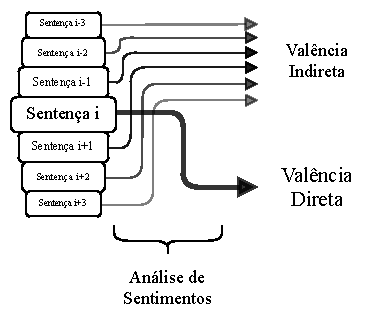
\includegraphics[width=0.5\linewidth]{figures/estimacao_valencia}
	
	Fonte: elaboração do autor
\end{figure}
 
Diante das limitações do LDA, como estratégia alternativa para mensurar o componente de Valência Indireta, foi adotado um procedimento de estimação baseado na correlação textual entre as setenças. Uma vez que expressões textuais estão temporalmente associadas e possuem uma ordenação que constitui seu sentido -- as expressões \textit{viver para trabalhar} e \textit{trabalhar para viver} possuem os mesmo termos, mas sentido distintos, por exemplo -- tomou-se o conjunto das 6 sentenças mais próximas da ocorrência de menção à Entidade -- as 3 sentenças que a precedem e as 3 sentenças que a sucedem -- como escopo de enquadramento. 

Na Figura 5 é possível visualizar o digrama de estimação dos componentes de Valência Indireta -- que advém do contexto de enquadramento e que correspode ao parâmetro $\lambda$ da Equação 3.3 -- e de Valência Direta -- que é extraído diretamente da sentença em que a Entidade é mencionada e que corresponde ao parâmetro $\beta$ da Equação 3.3. Assume-se que os limites de 3 sentenças posteriores e anterioes concentram a maior parte da correlação textual existente em discursos e que, se por um lado não são capazes de detectar analogias sutis, por outro, mensuram as porções de intencionalidade mais marcantes e assertivas do discurso.
 
De maneira sintética, os procedimentos de estimação do indicador de RWA proposto envolvem 2 etapas: 1) a estimação dos parâmetros da escala de Valores Autoritários para o indivíduo e 2) o cálculo final do RWA tomando a informação a priori e a resultante da escala de Valores Autoritários. Na primeira etapa são mensuradas as Valência da sentença de ocorrência e das sentenças vizinhas e da cada conjunto de raízes de Entidades Autoritárias -- conforme especifica o Quadro 1. Depois, esses resultados compõem os parâmetros da escala -- quantidade de Valores em que o agente se posicionou e quantidade de Valores com os quais manifestou adesão. Por fim, na segunda etapa, esses parâmetros são utilizados para restringir a distiruição a priori de RWA. E é a esperança condicional da distribuição a posteori que corresponde ao valor de RWA estimado, conforme a Equação 3.7.

\chapter{Prova de Mensuração}\label{resultados}

\section{Introdução}

A combinação de um passado autoritário recente, um resultado eleitoral que levou a presidência um candidato com plataforma de campanha fortemente marcada por traços iliberais \cite{hunter2019bolsonaro} e um sistema político de grandes dimensões tornam o Brasil um candidato para a investigação da expressão de autoritarismo em grandes grupos.

Ao longo dos últimos anos, representantes políticos que estabelecem identidade de campanha baseada na memória do regime militar ou no passado profissional como membros das forças de repressão do Estado têm angariado cada vez mais espaço nos pleitos eleitorais \cite{berlatto2015candidatos, berlatto2016policia}. A trajetória de crescimento do seu desempenho é precipitada ainda por eventos que aumentam a saliência da questão de segurança, como os ataques do PCC em 2006. Consistente oposição aos direitos humanos, filiação a partidos pequenos, defesa combativa do crime e enrijecimento das formas de controle social são elementos característicos do conteúdo da sua atuação \cite{berlatto2015candidatos, berlatto2016policia, faganellobancada, faganello2017voto}

Do ponto de vista das tentativas de identificação do fenômeno, a literatura angaria uma variedade de critérios de classificação que captam, em maior ou menor medida, traços autoritários típicos de alguns grupos de representantes. Candidatos das Forças de Repressão do Estado e Políticos das Forças de Segurança são duas tipologias utilizadas para identificar, entre candidatos e parlamentares, aqueles indivíduos que estão comprometidos com a narrativa de corporações militares e policiais \cite{berlatto2015candidatos,berlatto2016policia}. Já a Bancada da Bala refere-se a uma agremiação informal de parlamentares que fazem \textit{lobby} para indústria armamentista e tendem a compor um conjunto de forças conservadoras nas câmaras estaduais e federal \cite{faganellobancada,faganello2017voto}.

Além de Políticos das Forças de Segurança, congregações religiosas têm ganhado espaço no parlamento, em grande medida favorecidas por uma expansão do protestantismo no Brasil, e consolidada sua representação com base em pautas morais e uma associação cada vez mais estreita com formas dogmáticas de governo \cite{codato2015nova, do2016religiao}. \citeonline{do2016religiao} argumenta que houve, a partir dos anos 2000, um processo de transformação da cultura evangélica que cristalizou a politização de seus fiéis, instalando componentes ideológicos à direita do espectro político em seus imaginários. Como consequência, o eleitorado evangélico apresenta maior propensão ao voto corporativista \cite{netto2017dinheiro}. 

Em paralelo ao ganho de visibilidade de parlamentares evangélicos está o fato de que grupos políticos constituídos em torno do agronegócio, da mineração e da continuidade de dinastias políticas concentram uma porção expressiva de parlamentares na Câmara dos Deputados no Brasil \cite{congresso2016bancadas}. De fato, entre o pertencimento a famílias com passagem na política é um grande preditor de sucesso eleitoral e, entre os parlamentares mais jovens, os vínculos tendem a ser ainda mais intensos \cite{de2016familias}. Assim como os membros das Forças de Segurança e os Políticos Evangélicos, infere-se, com bases nas expectativas da literatura, discutida na seção 2.4, que setores produtivos primários e grupos familistas concentram maiores valores de RWA, em grande medida porque suas bases eleitorais espelham as precondições para gênese do autoritarismo. 

Em um espectro de estudos transversal, há trabalhos que utilizam discursos de candidatos e parlamentares como fonte para fazer inferências sobre posicionamentos relativos à questão agrária e indígena \cite{xavier2015senhores}, direitos reprodutivos \cite{miguel2017direito, santos2017debate}, sexualidade \cite{machado2013discursos, lacerda2016ideologia} e religiosidade \cite{gonccalves2016discurso}. Nessas investigações, conclusões acerca dos valores de tolerância e republicanismo adjacentes as falas compõem um mapa em formação das atitudes democráticas entre os representantes políticos. Contudo, nem todos os Políticos das Forças de Segurança, Candidatos das Forças de Repressão do Estado ou da Bancada da Bala, tal como Evangélicos, Ruralistas e Familistas, se opõem aos princípios democráticos, por vezes se limitam ao comportamento corporativista. Além disso, uma observação segmentada das falas impede a construção de índices de preconceito generalizado. 

Nas seções a seguir, serão detalhados os passos da construção de indicadores de RWA para os parlamentares brasileiros, a partir de suas falas, conforme os pressupostos e especificações definidas nas seções anteriores. Por fim, serão replicados testes para verificar as expectativas da literatura quanto aos parlamentares que tendem a expressas maior adesão à valores autoritários.

\section{Coletando e Organizando Dados}

Como forma de ampliar a transparência entre as atividades do plenário e os cidadãos, a Câmara dos Deputados possui o serviço de Dados Abertos, que conta com uma API de consulta pública, possibilitando a extração de dados de Blocos, Deputados, Eventos, Frentes, Legislaturas, Partidos, Proposições, Referências, Votações e Órgãos. A iniciativa, lançada em 2017 em consonância com a Lei de Acesso à Informação de 2011, permite o acesso fácil e o consumo em larga escala dos produtos do trabalho de transcrição e catalogação do Regimento Interno da Câmara dos Deputados.

No que diz respeito a velocidade de coleta, a documentação da API consta que, no período de 6:00 às 23:59, o Portal aceita 90 requisições por minuto e, das 00:00 às 5:59, 300. Foi por meio da API que os grandes volumes de dados de discursos de parlamentares foram extraídos de forma otimizada, utilizando \emph{framework} de raspagem de dados assíncrona. No período de elaboração dessa dissertação, as transcrições dos discursos realizados no plenário estavam disponíveis a partir dos anos 2000. Com isso, foi possível processar as falas proferidas entre a segunda metade da 51ª legislatura e meados da 56ª, permitindo a observação longitudinal de mais de 20 anos de atividade da Câmara dos Deputados, identificando de traços atitudinais em oradores que se manifestaram em pelo menos uma das seções.

\begin{center}
	Tabela 2 - Estatísticas de Oradores por Legislatura
	
	\vspace{0.4cm}
	
	\begin{tabular}{lccccccc}
		\toprule
		{}				& {51*}		& {52} 	& {53}	& {54}	& {55}	& {56**}	& {Total}	\\ \midrule
		{Deputados} 	& 642		& 629	& 646	& 671	& 633	& 545		& 3766		\\ 
		{Oradores} 		& 563		& 604	& 595	& 631	& 604	& 508		& 3556		\\ \midrule
		{Discursos} 	& 31377		& 77458	& 83629	& 83468	& 88265	& 24974		& 389171	\\ 
		\bottomrule
	\end{tabular}
	
	\vspace{0.6cm}
	
	* : dados coletados a partir de Janeiro de 2000; ** : dados coletados até Maio de 2020.
\end{center}

Na Tabela 2 é possível observar, em cada uma das legislaturas, o número de Deputados ativos -- contanto com eleitos e suplentes que assumiram o mandato em algum momento -- o número de Oradores -- Deputados ativos que realizaram ao menos algum discurso em alguma das seções -- e o volume de Discursos realizados. Descartando as legislaturas 51 e 56, por apresentarem dados restritos, é possível observar um movimento de crescimento da quantidade de discursos que não é acompanhado pelas flutuações no número de oradores. No total, ao longo do período de coleta, 389.171 discursos foram realizados por 3505 parlamentares\footnote{É importante ressaltar que, seguindo a estratégia metodológica de \citeonline{moreira2016palavra}, são considerados registros múltiplos em caso de indivíduos que foram eleitos para legislaturas distintas. Ou seja, um parlamentar é contado uma vez por legislatura para qual elegeu-se.}.

\begin{figure}[h]
	\caption{Quantis da Frequência de Realização de Discursos por Legislatura}
	\label{fig:quantis_discursos}
	\centering
	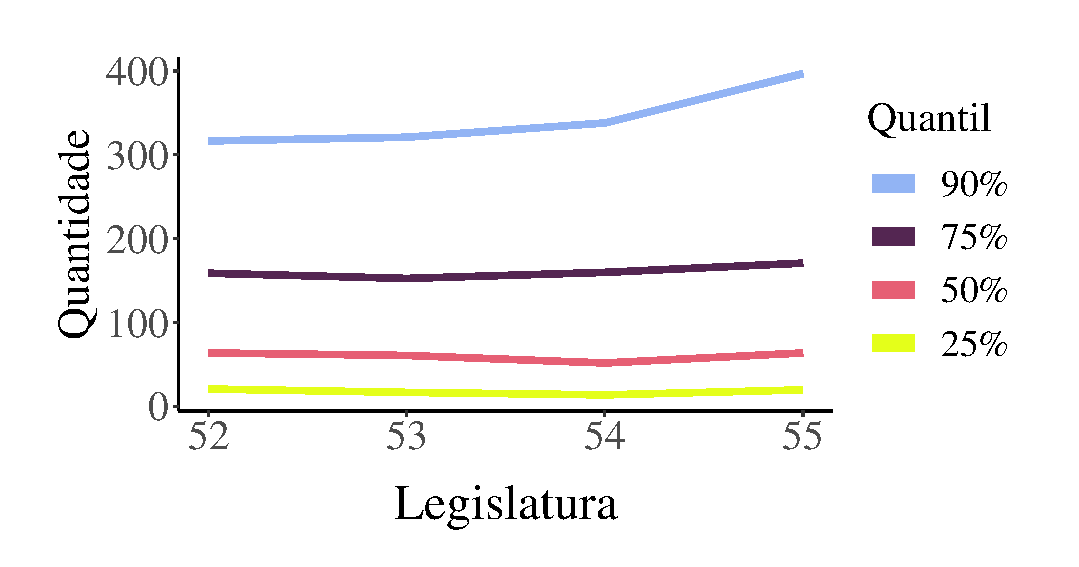
\includegraphics[width=.7\linewidth]{figures/quantis_discursos}
	
	Fonte: elaboração do autor
\end{figure}

Ainda no que diz respeito a tendência de ampliação do uso do espaço de fala, a Tabela 2 oferece indícios para inferir que esse processo decorre da concentração de pronunciamentos em uma porção restrita de parlamentares. A despeito das flutuações nos valores da mediana, os quantis mais elevados de frequência têm seus valores ampliados ao longo da série histórica. Essa dinâmica acentua um fato documentado pela literatura, e reforçado pela Figura 6, de que uma minoria de Deputados concentra grande espaço nos pronunciamentos do plenário \cite{moreira2016palavra}. Em todas as legislatura, é possível identificar uma distribuição de hiper-concentrada nos valores mais baixos e uma longa calda onde estão incluídos os parlamentares mais comunicativos.    

\begin{figure}[!htb]
	\caption{Distribuição da Realização de Discursos por Legislatura}
	\centering
	
	\hspace{.05\linewidth}
	\begin{minipage}[b]{0.3\textwidth}
	\textbf{Legislatura 51}
	\label{fig:dens_legis_51}
	\centering
	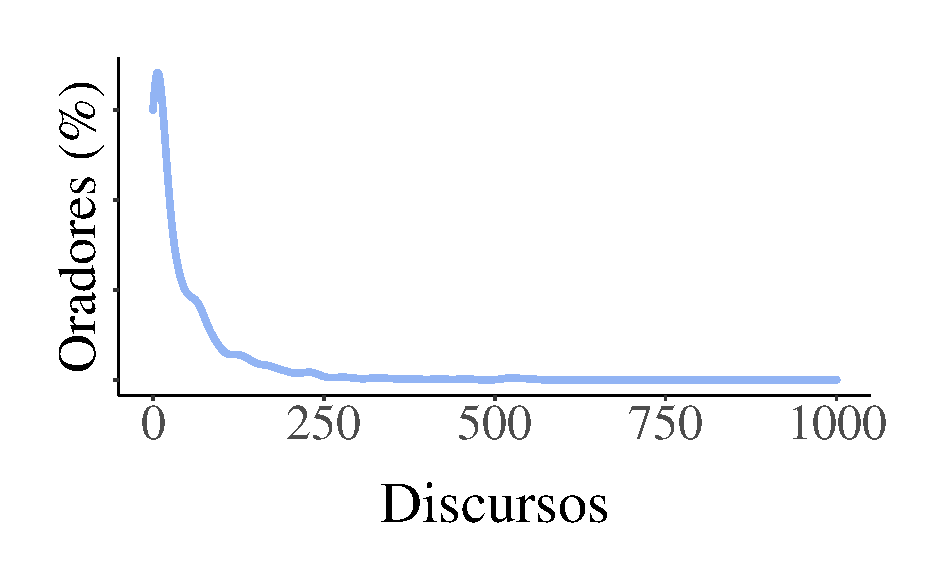
\includegraphics[width=1\linewidth]{figures/dens_oradores_51}
	
	\end{minipage}
	\hspace{.05\linewidth}
	\begin{minipage}[b]{0.3\textwidth}
		\textbf{Legislatura 52}
		\label{fig:dens_legis_52}
		\centering
		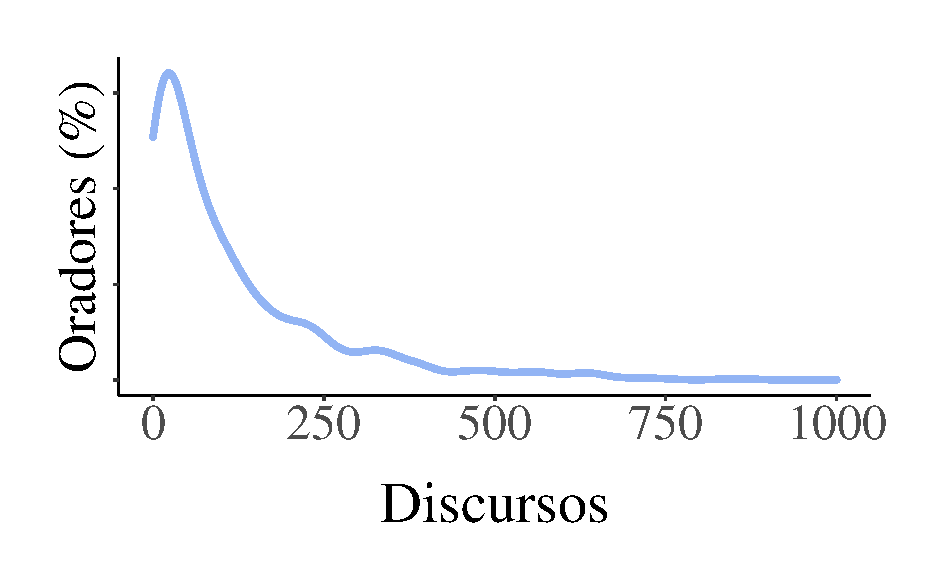
\includegraphics[width=1\linewidth]{figures/dens_oradores_52}
		
	\end{minipage}
	\\
	\hspace{.05\linewidth}
	\begin{minipage}[b]{0.3\textwidth}
		\textbf{Legislautra 53}
		\label{fig:dens_legis_53}
		\centering
		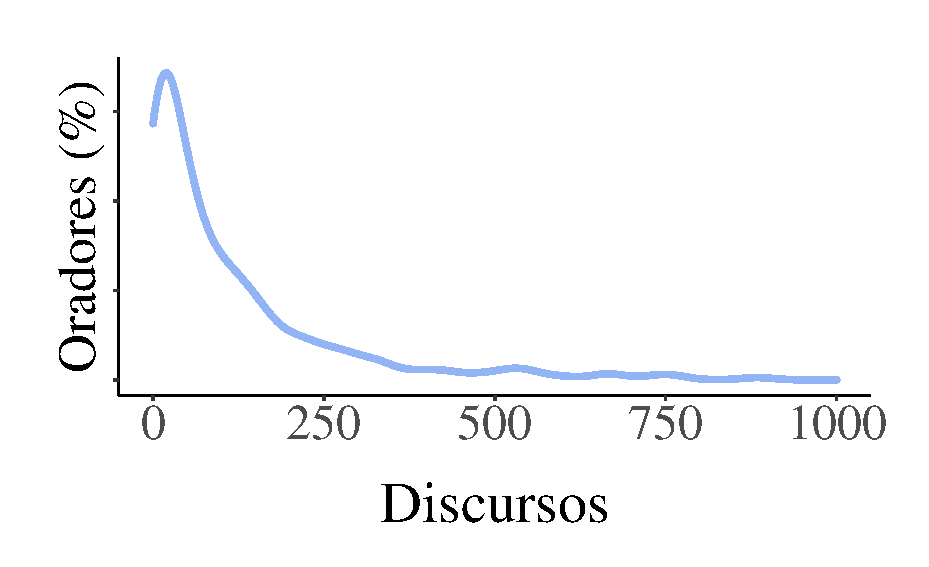
\includegraphics[width=1\linewidth]{figures/dens_oradores_53}
		
	\end{minipage}
	\hspace{.05\linewidth}
	\begin{minipage}[b]{0.3\textwidth}
		\textbf{Lgislatura 54}
		\label{fig:dens_legis_54}
		\centering
		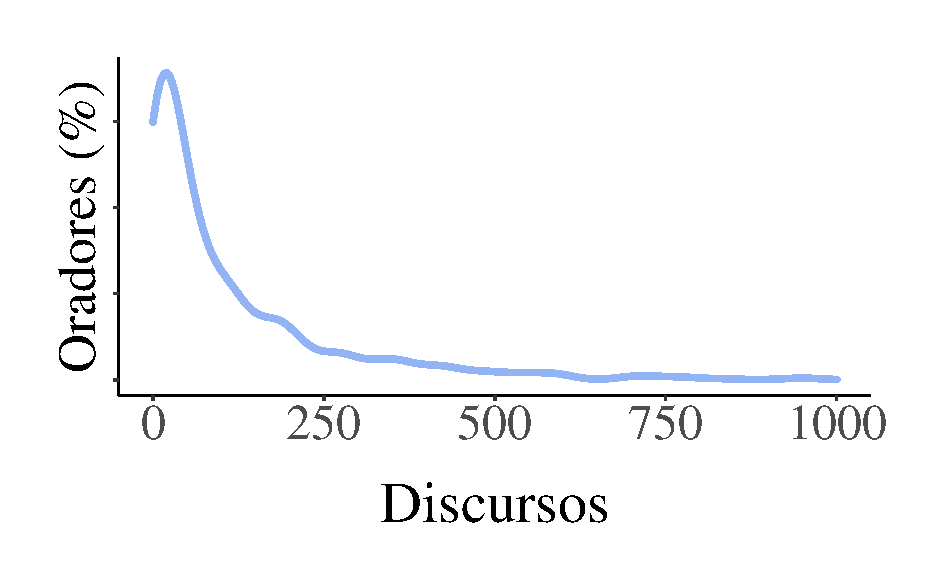
\includegraphics[width=1\linewidth]{figures/dens_oradores_54}
		
	\end{minipage}
	\\
	\hspace{.05\linewidth}
	\begin{minipage}[b]{0.3\textwidth}
		\textbf{Legislautra 55}
		\label{fig:dens_legis_55}
		\centering
		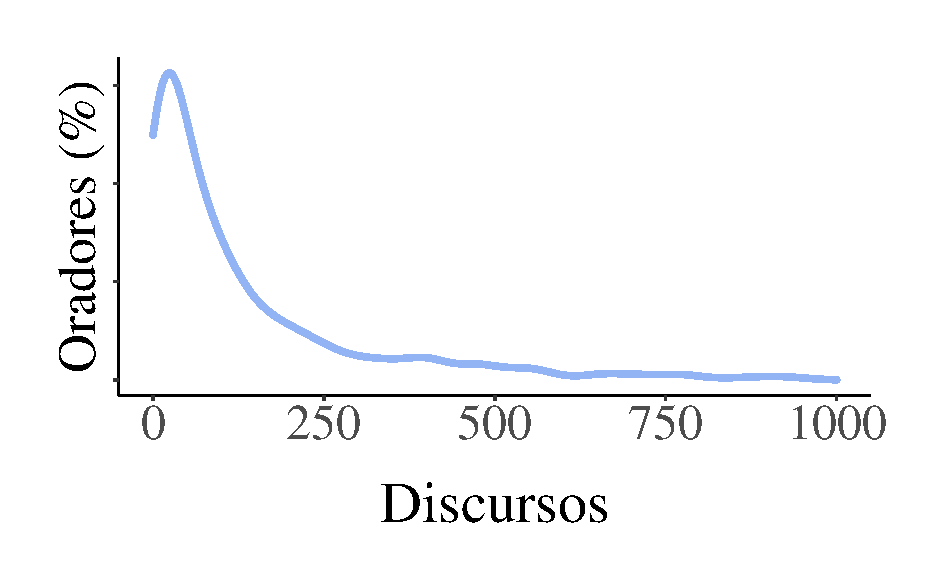
\includegraphics[width=1\linewidth]{figures/dens_oradores_55}
		
	\end{minipage}
	\hspace{.05\linewidth}
	\begin{minipage}[b]{0.3\textwidth}
		\textbf{Legislatura 56}
		\label{fig:dens_legis_56}
		\centering
		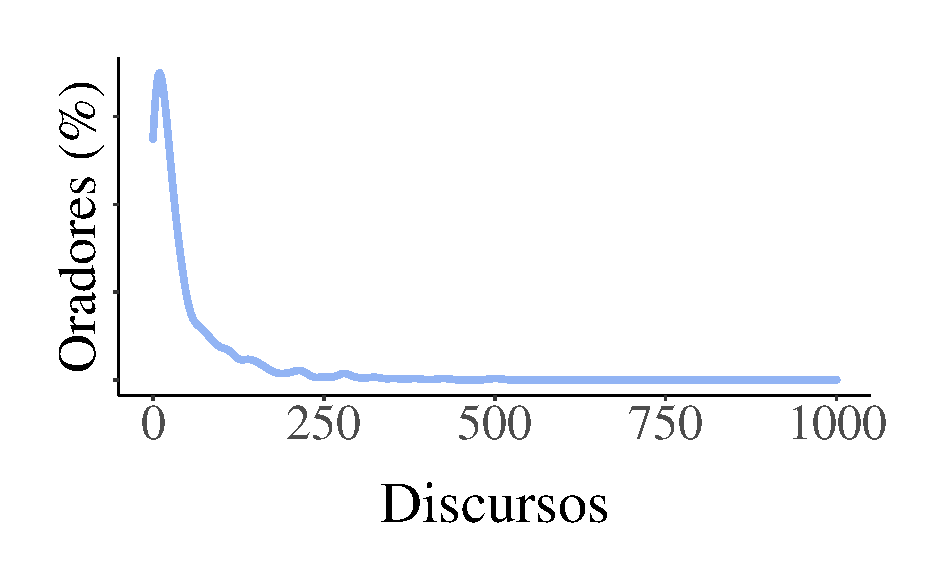
\includegraphics[width=1\linewidth]{figures/dens_oradores_56}
		
	\end{minipage}	

	Fonte: elaboração do autor
	\begin{flushleft}
		Nota: O limite das abcissas dos gráficos foi fixado com o propósito de facilitar a visualização. Os pontos de máximo para as legislaturas são: 1186, 51; 2383, 52; 5965, 53; 2268, 54; 1829, 55 e 501, 56. 
	\end{flushleft} 
\end{figure}

Além de observar a frequência de pronunciamentos parlamentares, para a estimação do indicador de RWA proposto, é necessário observar a ocorrência de raízes de palavras que mapeiam cada uma das dimensões do autoritarismo, conforme foi especificado no Quadro 1. Na Figura 8 é possível observar que a quantidade de parlamentares que mencionaram em seus discursos termos pertencentes a cada dimensão. É importante ressaltar que o gráfico não representa os valores de Submissão à Autoridade, Agressividade Autoritária e Convencionalismo em si, mas a ocorrência de termos que tornam possível estimar o posicionamento latente do parlamentar em relação aos Valores Autoritários.

\begin{figure}[h]
	\caption{Quantidade de Oradores por Dimensão de RWA}
	\label{fig:qtd_deps_rwa}
	\centering
	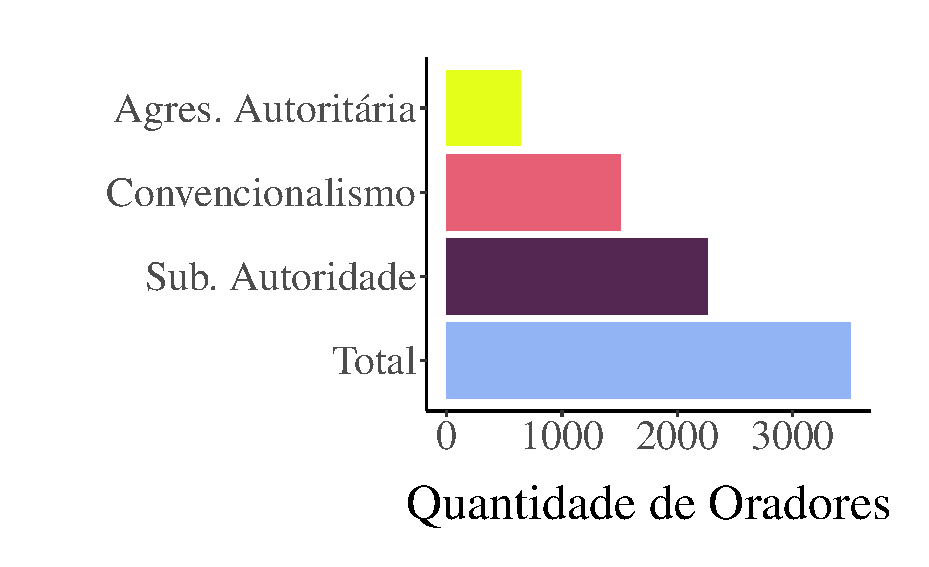
\includegraphics[width=.6\linewidth]{figures/qtd_oradores_rwa}
	
	Fonte: elaboração do autor
	\begin{flushleft}
	Nota: Os valores do número máximo de discursos com menções a raízes que compõem as dimensões do RWA entre parlamentares são, respectivamente: Submissão à Autoridade, 3232; Convencionalismo, 1455; Agressividade Autoritária, 537. 
	\end{flushleft} 	
\end{figure}

Ainda sobre a Figura 8, pode-se constatar que, do total de 3505 oradores identificados entre as legislaturas 51 e 56, 2260 -- 64{\%} -- fizeram referência a termos que compõem dimensão de Submissão à Autoridade, 1506 -- 42{\%}, à Convencionalismo e 637 -- 18{\%}, à Agressividade Autoritária. Os números refletem a saliência dos subcomponentes de cada dimensão. Enquanto Ufanismo e Radicalismo Religioso são tópicos populares -- tanto em manifestações favoráveis ou contrárias -- o Punitivismo, Patriarcalismo e Rejeição à Diversidade representam pautas restritas, ligadas a agenda de um número relativamente pequeno de parlamentares. Considerando todas as dimensões, apenas 40 -- 1,1{\%} -- oradores se manifestaram sobre todas os componentes do RWA, reforçando o fato de que a informação atitudinal obtida por meio de dados textuais carrega as características de um fenômeno latente e parcialmente observado. 

Na seção seguinte, serão apresentados os procedimentos para estimativa de RWA entre parlamentares brasileiros a partir dos seus pronunciamentos no plenário da Câmara dos Deputados.

\section{Estimando Autoritarismo entre Deputados}

Observando a distribuição da Escala de Valores Autoritários, a qual mensura a quantidade de Valores Autoritários com os quais um indivíduo manifestou adesão, é possível constar às expectativas quanto a sua esparsidade. Na Figura 9 constata-se que, apesar de um pouco menos da metade -- 42{\%}-- dos oradores da Câmara dos Deputados terem manifestado adesão por pelo menos um dos valores, apenas em uma fração reduzida dos casos parlamentares pontuaram elevados valores na escala. De fato, nenhum dos agentes analisados alcançou o valor máximo da escala, 8, e apenas um único indivíduo conseguiu atingir a marca de 7 pontos.

\begin{figure}[h]
	\caption{Distribuição da Escala de Valores Autoritários}
	\label{fig:scale_auth_val}
	\centering
	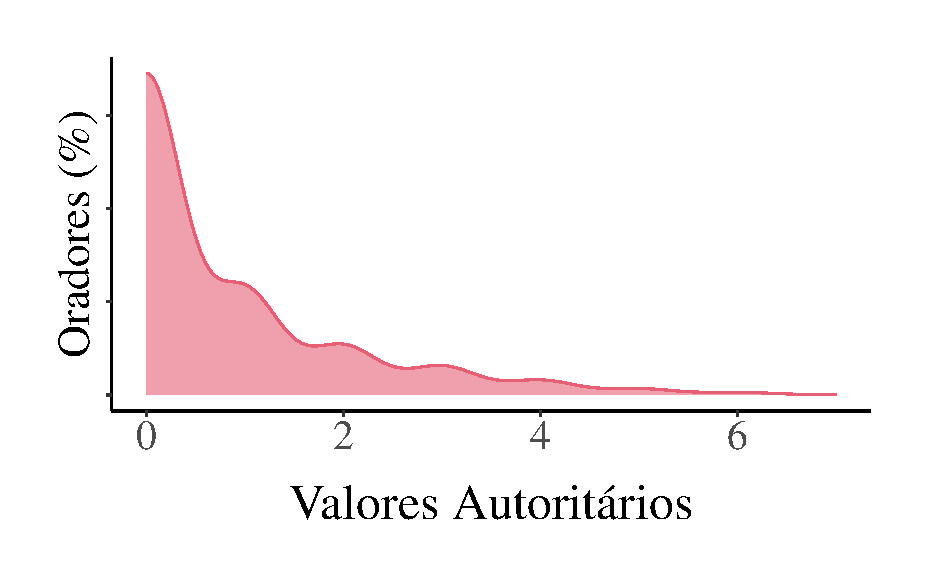
\includegraphics[width=.6\linewidth]{figures/scale_auth_val}
	
	Fonte: elaboração do autor	
\end{figure}

O lugar de destaque infeliz na escala é ocupado pelo Deputado Federal André Moura, líder do PSC. Em sua trajetória, o parlamentar apresenta uma defesa intransigente da Igreja Evangélica e das corporações policiais, para os quais dedica boa parte de sua atividade como legislador. Diversas proposições e falas na Câmara reforçam seu apoio incondicional à greves de agentes de segurança, aumento salários e de efetivo. Em paralelo, o Deputado se mobilizou ativamente contra mudanças na legislação que assinalavam divergências com instituições tradicionais. Em 2013, liderou o impretamento de mandado de segurança contra o reconhecimento da união estável entre pessoas do mesmo sexo.  	 

No dia 5 de Junho de 2013, na ocasião de uma manifestação ``em defesa da família tradicional, da liberdade de expressão e de culto'' em frente ao Congresso, declarou:

\begin{quotation}
	Esse evento é organizado pelo segmento evangélico do País. Todas as igrejas do segmento evangélico se reuniram para realizar esse evento e, acima de tudo, para demonstrar a posição das famílias em defesa dos princípios cristãos, em defesa da família brasileira, que é o alicerce principal do nosso País.[...] Com a participação de milhares de pessoas, podemos ouvir a manifestação de apoio [...] aos princípios cristãos, a família e o cidadão.
\end{quotation}

As manifestações de RWA realizadas pelo parlamentar podem ainda ser observadas a partir da conjugação de valores Convencionalistas e de Agressividade Autoritária. 

Em discurso realizado do dia 2 de Agosto de 2011, apresentou proposta de redução da maioridade penal para 16 anos como forma controle da criminalidade. Como efeito esperado da medida, assinalou que por causa do enrijecimento da punição, jovens teriam seu ingresso na vida do crime contido por causa da ampliação do medo de ser pego. Já em 17 de Dezembro de 2013, apresentou proposta da obrigatoriedade do trabalho para detentos. Como defesa da proposta, o parlamentar argumentou:

\begin{quotation}
	 Naturalmente, o PL 4.853, de 2012, de nossa autoria, não resolve todos os problemas do sistema prisional brasileiro. Porém, tem como grande apelo proporcionar aos condenados pela Justiça a oportunidade de encarar a pena com esforço digno, que lhes remunera e os resgata do crime, pois esta é a grande virtude do trabalho honesto: elevar a autoestima do homem.
\end{quotation}

A conjugação de penas mais duras e o trabalho como instrumento de dignificação do humano reforçam, simultaneamente, a narrativa de que a integridade do tecido social depende de uma dupla agência que envolve a submissão às autoridade e ao lugar social de força produtiva e do reforço da punição como método de castração de impulsos desviantes.

Na Figura 10 é possível visualizar a distribuição do RWA estimado para os 3505 Oradores ao longo das legislaturas 51 até 56. Segundo essa escala, o valor médio do RWA para os Deputados brasileiros é 1.87, levemente superior a média da distribuição a priori, porém a diferença não é estatisticamente significativa\footnote{A média da distribuição a priori é 1.62, 0.25 pontos abaixo do RWA dos Deputados brasileiros, indicando, portando, uma diferença de aproximadamente meio desvio padrão.}. Ao longo das legislaturas, a média variou de maneira sutil entre 2, valor máximo atingido na legislatura 53, e 1.78, valor mínimo atingido na legislatura 56. 

A conjugação de baixas variações na média, distribuição bem menos concentrada nos valores menores e o fato de que em toda a série histórica nenhum parlamentar superou os 4 pontos nas escala de RWA sugerem que o autoritarismo manifesto na Câmara dos Deputados ao longo dos últimos 20 anos é consideravelmente mais limitado do que na população em geral. Em comparação a Figura 1, não é possível observar a existência de uma longa cauda que comporta super radicais de extrema-direta, os quais tendem a compor bolhas autoritárias.


\begin{figure}[h]
	\caption{Distribuição da Escala Alternativa de RWA}
	\label{fig:scale_rwa}
	\centering
	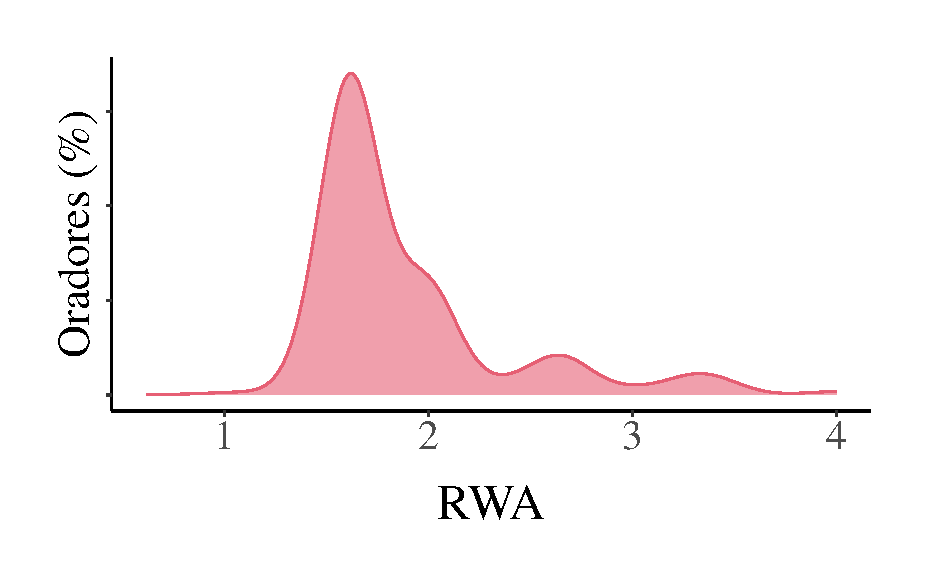
\includegraphics[width=.6\linewidth]{figures/scale_rwa}
	
	Fonte: elaboração do autor	
\end{figure}

Apesar o processo relativamente contínuo, um apontamento relevante sobre a dinâmica de expressão de valores autoritários é no que diz respeito a dispersão atitudinal, há uma variação considerável entre algumas das legislaturas. Como é possível constatar na Figura 11, entre as legislaturas 51 e 53 há um achatamento das curvas, indicando um aumento na variabilidade de posicionamentos. A partir de então, a distribuição volta, paulatinamente, a se concentrar. Comparando o desvio-padrão das distribuições, a legislatura 53 é 27{\%} mais dispersa que a 51 e 37{\%} mais dispersa que a 56.

Sobre esse padrão, é possível identificar na literatura um grande número de referências ao crescimento da Bancada Evangélica na primeira décadas do século XXI. De forma menos consistente, algumas evidências sugerem, para as últimas legislaturas, redução da saliência do conservadorismo moral e uma conversão à direita do espectro político. Ainda sim, não é possível afirmar com clareza que as variações na dispersão dos valores de RWA se devem a movimentos endógenos de Bancadas e Frentes Parlamentares.     

\begin{figure}[!htb]
	\caption{Distribuição da Escala Alternativa de RWA por Legislatura}
	\centering
	
	\hspace{.05\linewidth}
	\begin{minipage}[b]{0.3\textwidth}
		\textbf{Legislatura 51}
		\label{fig:dense_rwa_51}
		\centering
		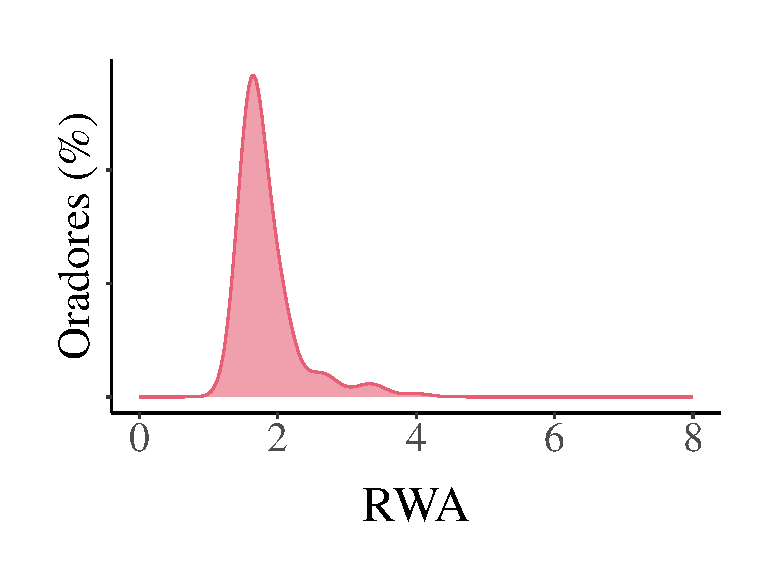
\includegraphics[width=1\linewidth]{figures/dense_rwa_51}
		
	\end{minipage}
	\hspace{.05\linewidth}
	\begin{minipage}[b]{0.3\textwidth}
		\textbf{Legislatura 52}
		\label{fig:dense_rwa_52}
		\centering
		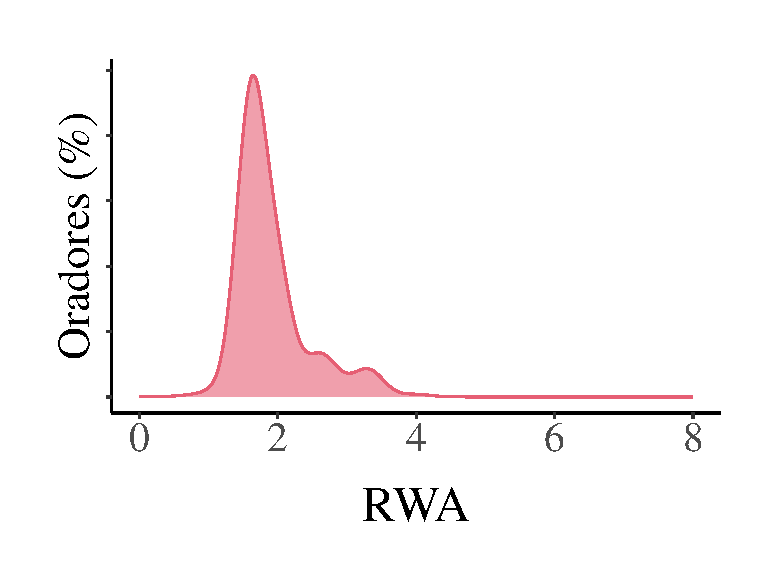
\includegraphics[width=1\linewidth]{figures/dense_rwa_52}
		
	\end{minipage}
	\\
	\hspace{.05\linewidth}
	\begin{minipage}[b]{0.3\textwidth}
		\textbf{Legislautra 53}
		\label{fig:dense_rwa_53}
		\centering
		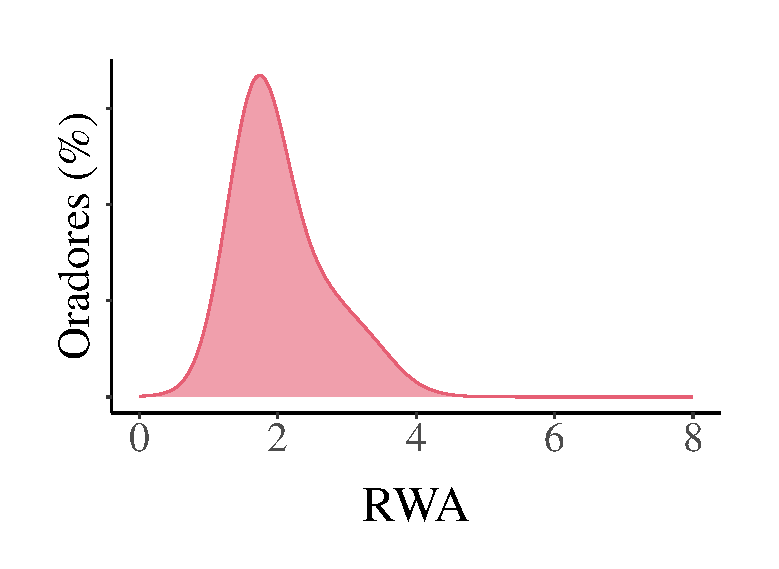
\includegraphics[width=1\linewidth]{figures/dense_rwa_53}
		
	\end{minipage}
	\hspace{.05\linewidth}
	\begin{minipage}[b]{0.3\textwidth}
		\textbf{Lgislatura 54}
		\label{fig:dense_rwa_54}
		\centering
		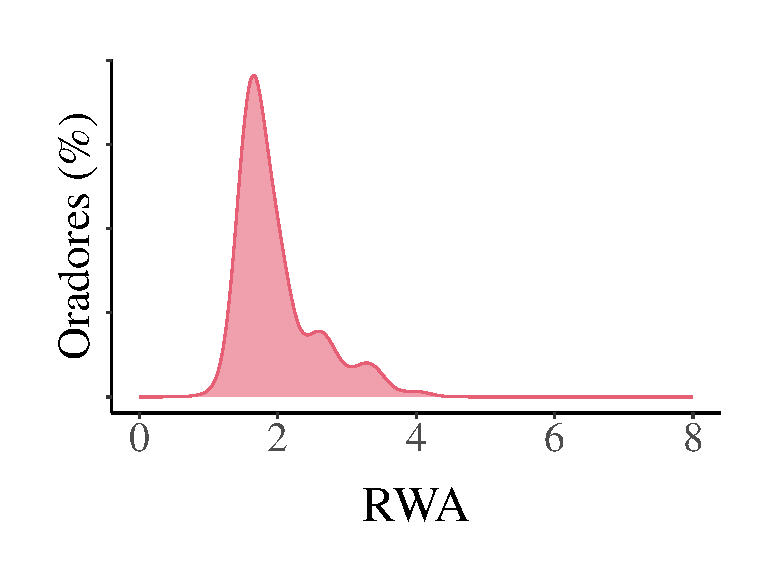
\includegraphics[width=1\linewidth]{figures/dense_rwa_54}
		
	\end{minipage}
	\\
	\hspace{.05\linewidth}
	\begin{minipage}[b]{0.3\textwidth}
		\textbf{Legislautra 55}
		\label{fig:dense_rwa_55}
		\centering
		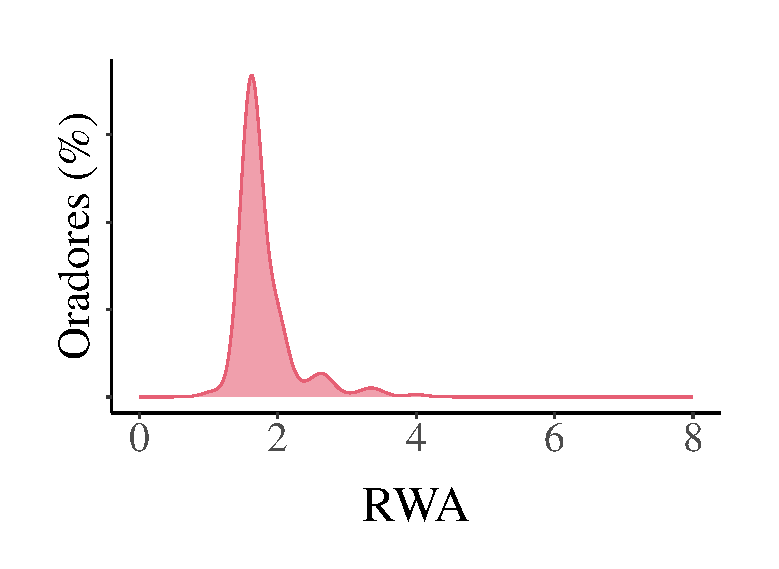
\includegraphics[width=1\linewidth]{figures/dense_rwa_55}
		
	\end{minipage}
	\hspace{.05\linewidth}
	\begin{minipage}[b]{0.3\textwidth}
		\textbf{Legislatura 56}
		\label{fig:dense_rwa_56}
		\centering
		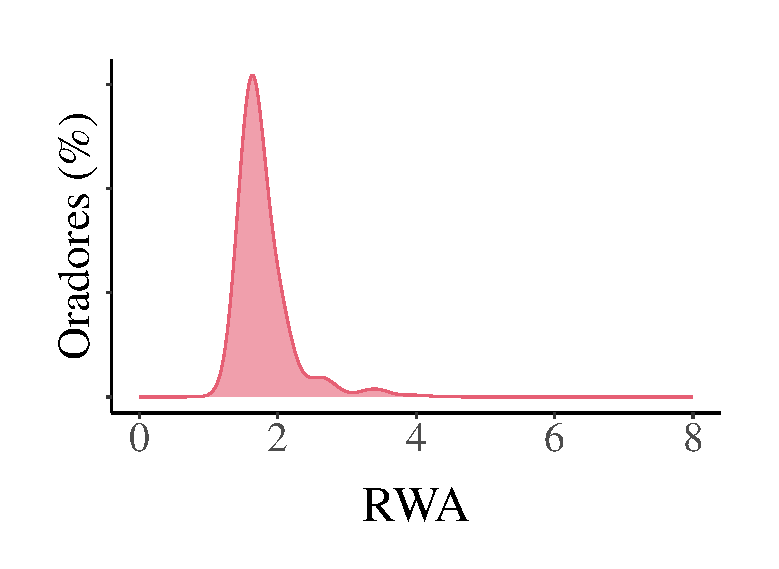
\includegraphics[width=1\linewidth]{figures/dense_rwa_56}
		
	\end{minipage}	
	
	Fonte: elaboração do autor
	\begin{flushleft}
		Nota: Os desvios-padrão para cada legislatura correspondem, respectivamente, a: 0.43, 51\textbf{;} 0.50, 52\textbf{;} 0.59, 53\textbf{;} 0.54, 54\textbf{;} 0.40, 55 \textbf{e} 0.37, 56. 
	\end{flushleft} 
\end{figure}

\section{Avaliando Autoritarismo por Segmentos de Parlamentares}

Conforme foi discutido, a manifestação de RWA é condicionada por características individuais. Apesar da ausência de variações significativas na expressão de atitudes autoritárias ao longo das legislaturas, é possível identificar segmentos de parlamentares que concentram maior número de indícios de comportamento anti-democrático. Mesmo que constituam um grupo pequeno em meio a população de parlamentares que já passaram pela Câmara, pastores evangélicos e ex-membros das Forças de Segurança -- militares e policiais -- destacam-se nos top 10 de oradores com maiores valores no indicador de autoritarismo. 5 dos 10 lugares -- 2 deles por pastores e 3 por militares -- são ocupados por esses tipos de representantes.

Uma ressalva importante é que as categorias de Políticos da Segurança e Políticos Evangélicos fazem referência ao uso, pelos parlamentares, de identificadores que possibilitam estabelecer a conexão entre suas candidaturas e as entidades que sugerem representar. Em sua investigação sobre o desempenho eleitoral de Candidatos das Forças Repressivas do Estado, Berlatto, Codato e Bolognesi
\citeonline{berlatto2015candidatos, berlatto2016policia} adotaram como critério de classificação a origem profissional. Contudo, a estratégia utilizada pelos autores deixa de fora alguns grandes casos de deputados que possuem passado profissional na polícia ou no exército, mas que, por estarem afastados há algum tempo, declararam outra ocupação, vide exemplo do Coronel Chrisóstomo, eleito na legislatura 56 pelo estado de Rondônia, com uma plataforma de campanha militarista e anti-imigratória.

A alternativa adotada para contornar o problema, que se estende para o caso de Políticos Evangélicos, foi utilizar acrescentar a presença de termos que remetam a hierarquia policial ou militar, tal como designações religiosas, no nome de urna dos candidatos aos critérios de classificação. Essa solução metodológica replica a implementação realizada por \citeonline{netto2017dinheiro}, nos quais os autores utilizaram a classificação baseada no nome de urna como atalho para candidatos evangélicos e mensurar o efeito do pertencimento à corporação religiosa no sucesso eleitoral.

Explorando as especificidades dessa dinâmica, na Figura 12 é possível observar que, em comparação àqueles que possuem outras ocupações, Políticos Evangélicos apresentam média superior de RWA, indicando que há maior tendência de expressão de autoritarismo entre os integrantes do grupo. Já em relação aos Políticos da Segurança, apresentam média semelhante aos outros Deputados e apenas no quantil de 95{\%} pode-se apontar uma concentração relativa maior. Ou seja, enquanto que Políticos Evangélicos aparecem com valores de RWA sistematicamente maiores, Políticos da Segurança destacam-se apenas entre os super-autoritários.   

\begin{figure}[h]
	\caption{Distribuição da Escala Alternativa de RWA por Grupo de Parlamentares}
	\label{fig:rwa_grupos}
	\centering
	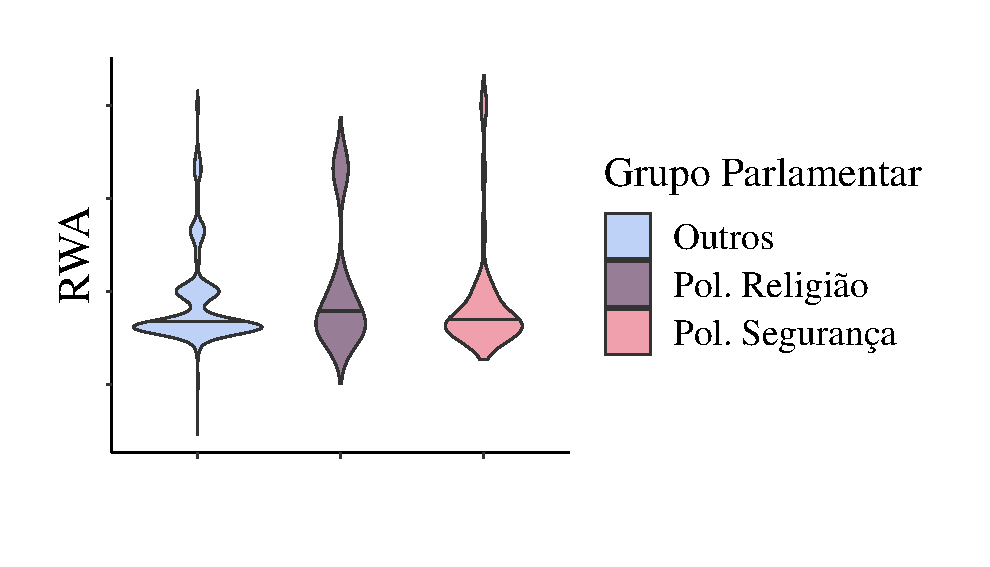
\includegraphics[width=.7\linewidth]{figures/rwa_grupos}
	
	Fonte: elaboração do autor	
\end{figure}

Tomando como referencial o trabalho de mapeamento da \citeonline{congresso2016bancadas}, a qual identificou os Deputados em exercício do mandato que integravam as 11 bancadas mais poderosas do Congresso no período da legislatura 55, a Figura 13 apresenta os valores padronizados de RWA por bancada. Conforme as expectativas, os parlamentares que integram a pauta dos Direitos Humanos apresentam os menores níveis de autoritarismo, com 0.35 desvios-padrão abaixo da média. O grupo é seguido pela bancada Sindical, com o qual compartilha o posicionamento à esquerda do espectro político.

Um dos destaques no gráfico se deve a posição relativa das bancadas da Bala e Evangélica. A duas são apontadas pela literatura como grupos preponderantes na manifestação de conservadorismo moral e demandas repressivas no campo da segurança pública, mas que, na distribuição, concentraram-se na parte média da escala. Outro ponto relevante é o fato de que os grupos dos parlamentares familistas e associados à atividades do setor primário, assinalados, respectivamente, pela bancada dos Parentes, Ruralistas e Mineradores (os dois últimos representam agremiações de produtores de commodities), sobrepuseram à média em 0.05, 0.08 e 0.15 desvios-padrão, ocupando o espaço mais autoritário na escala.
  
\begin{figure}[h]
	\caption{Distribuição da Escala Alternativa de RWA por Bancadas}
	\label{fig:rwa_bancadas}
	\centering
	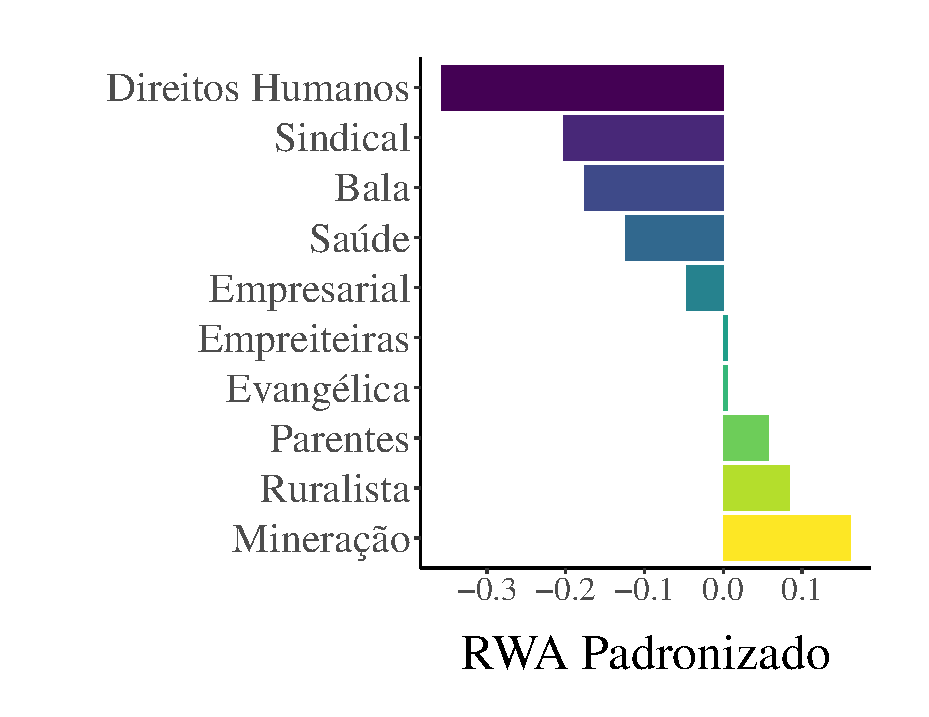
\includegraphics[width=.6\linewidth]{figures/rwa_bancadas}
	
	Fonte: elaboração do autor	
\end{figure}

Os resultados contraintuitivos em relação aos Políticos da Segurança, que a priori poderiam ser interpretados como a rejeição da hipótese sobre a relação entre violência e autoritarismo, sugerem, sobretudo, limitações do indicador alternativo de RWA. As duas principais suspeitas quanto as fontes de ruído são: i) má identificação das Raízes textuais associadas às falas sobre o fenômeno explicitada no Quadro 1 e ii) estimação inadequada da Escala de Valores Autoritários, que é sensível a vieses presentes no modelo de identificação da polaridade das sentenças. Ou seja, a melhora na precisão do indicador alternativo de RWA, proposto nessa dissertação, passa por uma análise mais acurada da semântica e das formas de manifestação de adesão em discursos que envolvem valores de Punitivismo. 

Como síntese dos resultados apresentados, pode-se estabelecer que: i) o indicador proposto nesta dissertação apresenta limitações, mas apresentou aderência à maioria das expectativas da literatura que se utiliza das escalas usuais (F e RWA); ii) a média de autoritarismo não variou significativamente ao longa das legislaturas no Brasil, indicando que trata-se de um fenômeno estável no longo prazo; iii) essa estabilidade, contudo, é complexificada pelo fato de que algumas legislaturas apresentam grandes variações na dispersão de RWA entre os Deputados, o que sugere a possibilidade de polarização parlamentar em torno de pautas democráticas; iv) a composição representativa é um elemento de forte segmentação de políticos por grau de adesão à democracia, uma vez que grupos de parlamentares podem apresentar tendências opostas quanto a propensão à manifestação de atitudes autoritárias. 

\chapter{Conclusão}

As investigações sobre causas e efeitos do autoritarismo vêm se tornando cada vez mais populares na literatura e na mídia. Em grande medida, a principal motivação desse fenômeno está na emergência, cada vez mais intensa, de lideranças políticas autoritárias em regimes democráticas. Nesse contexto, a possibilidade de derrocada das instituições que garantem a estabilidade do regime promovidas por aqueles eleitos pelo voto popular lançou luz para a necessidade de observar o autoritarismo em todas as suas camadas, inclusive sobre as atitudes e comportamentos das elites políticas no poder. 

Porém, se por um lado a literatura em psicologia política conta com instrumentos consistentes e amplamente testados para mensurar propensão ao autoritarismo, por outro, nos trabalhos em Ciência Política que envolvem o tema, pesquisadores ainda contam com ferramentas limitadas para classificação de agentes políticos autoritários. Isso se deve principalmente ao fato de que as escalas F e RWA, propostas respectivamente por \citeonline{adorno1950authoritarian} e \citeonline{altemeyer1981right}, envolvem a aplicação de questionários sensíveis e o acesso direto às lideranças políticas de movimentos sociais e parlamento é limitado. Portanto, para medir o nível de adesão a narrativa de que ``o mundo é um lugar hostil e perigoso, no qual a segurança coletiva, a estabilidade e a ordem são indispensáveis a qualquer custo'', pesquisadores recorrem a heurísticas ou inferências com bases em dados alternativos.

Apesar do grande volume de conhecimento produzido sobre o tema, observação limitada do autoritarismo no nível individual têm como consequência o eclipse de agentes políticos autoritários que não ganharam relevância o suficiente para tornarem-se objetos de pesquisa. Dada essa lacuna na literatura, foi proposto, nessa dissertação, um indicador alternativo de autoritarismo baseado na análise automatizada de discursos autoritários que, por meio de algoritmos de Processamento de Linguagem Natural, permite classificação em larga escala e é aderente aos instrumentos tradicionais da psicologia política. 

O indicador é fruto da composição de uma distribuição a priori -- definida a partir de dados de respostas para o questionário proposto por \citeonline{altemeyer1981right} -- e uma distribuição de verossimilhança, definida pela Escala de Valores Autoritários, que mede a adesão ou rejeição a 8 conjunto de valores típicos no discurso autoritário. Para a operacionalização do indicador, foram definidos i) um dicionário de Raízes Textuais, que mapeia o campo semântico de cada um dos valores, e ii) um modelo de Análise de Sentimentos, capaz de mensurar a polaridade das sentenças associadas a cada Raiz Textual.

Por fim, como forma de validar o indicador alternativo de RWA proposto, algumas expectativas da literatura foram retestadas tomando como base os parlamentares da Câmara dos Deputados no Brasil. Para isso, foram extraídos discursos realizados entre Janeiro de 2000 até Maio de 2020 no plenário e mensurados os valores de autoritarismo de 3556 indivíduos. Quanto as hipóteses avaliadas, foram observados se parlamentares i) das Forças de Segurança, ii) representantes de Congregações Religiosas, iii) membros de dinastias familiares na política e iv) associados a produção de \emph{commodities} apresentavam maior expressão de autoritarismo que a média dos Deputados.

Os resultados apresentaram correspondência parcial com as expectativas da literatura e 3 das 4 hipóteses foram confirmadas. Esses indicativos sugerem que o indicador proposto apresenta boa aderência com as medidas obtidas por meio de instrumentos mais precisos, porém há limitações quanto a identificação de adesão ao Punitivismo, dado que Políticos das Forças de Segurança apresentaram valores de RWA próximo da média de outros parlamentares. Dessa forma, pode-se concluir que, apesar de não resolver de forma definitiva os problemas enfrentados por pesquisas sobre autoritarismo na política, o indicador oferece um bom ponto de partida para novas explorações no campo de pesquisa.


% ----------------------------------------------------------
% ELEMENTOS PÓS-TEXTUAIS
% ----------------------------------------------------------
\postextual
% ----------------------------------------------------------

% ----------------------------------------------------------
% Referências bibliográficas
% ----------------------------------------------------------
\bibliography{bibli}

% ----------------------------------------------------------
% Glossário
% ----------------------------------------------------------
%
% Consulte o manual da classe abntex2 para orientações sobre o glossário.
%
%\glossary

% ----------------------------------------------------------
% Apêndices
% ----------------------------------------------------------

Apêndices

%---------------------------------------------------------------------
% INDICE REMISSIVO
%---------------------------------------------------------------------
\phantompart
\printindex
%---------------------------------------------------------------------

\end{document}
